\section{Was ist eine Funktion?}
\subsection{Einführungsaufgaben}
\begin{enumerate}
    \item G. ist Weltraumschrotthändlerin. Mit ihrer Weltraumschrottwaage wiegt sie den Schrott und ordnet dem jeweiligen Gewicht einen Preis zu. Es wird also einer ersten Grösse $x$ (Gewicht) eine zweite Grösse $y$ (Preis) zugeordnet. \\
          Man sagt auch: Der Preis hängt \emph{funktional} von dem Gewicht ab, weil jedem möglichen Gewicht des Weltraumschrotts in eindeutiger Weise ein Preis zugeordnet wird.
          \begin{enumerate}
              \item Was für Zahlen kommen hier für die Grösse $x$ in Frage? Und was für Zahlen für die Grösse $y$?
              \item Was denken Sie, nach was für einer Regel oder Formel wird eigentlich der Preis aus dem Gewicht bestimmt? Wie würden Sie das als Verkäuferin oder Verkäufer tun?
          \end{enumerate}
    \item Nico behauptet von sich, dass er in Windeseile jede beliebige Zahl quadrieren kann.
          Man kann ihm also einfach irgendeine Zahl $x$ nennen, und er berechnet dann daraus
          $y$, das dem $x$ zugeordnete Quadrat. Man sagt auch: Die Zahl $y$ hängt
          \emph{funktional} von der Zahl $x$ ab, weil jeder möglichen Zahl $x$ in eindeutiger
          Weise ihr Quadrat zugeordnet ist.

          \begin{enumerate}
              \item Was für Zahlen kommen hier für die Grösse $x$ in Frage? Und was für Zahlen
                    für die Grösse $y$?
              \item Mit welcher Formel in $x$ und $y$ würden Sie die Zuordnung ausdrücken,
                    die Nico ausführt?
          \end{enumerate}
    \item Martina hat einen langen, schmalen Papierstreifen vor sich. Zum Zeitvertreib faltet sie ihn ein erstes Mal mittig, dann ein zweites Mal, dann ein drittes Mal, und so weiter. Mit jeder weiteren Faltung wird der Stapel dicker und sperriger.

          Irgendwann fragt sich Martina, wie eigentlich die Dicke des Stapels von der Anzahl der Faltungen abhängt. Es wird also einer ersten Grösse $x$ (Anzahl der Faltungen) eine zweite Grösse $y$ (Dicke des Stapels) zugeordnet. Man sagt auch: Die Dicke des Stapels hängt \emph{funktional} von der Anzahl der Faltungen ab, weil jeder möglichen Anzahl der Faltungen in eindeutiger Weise eine Dicke zugeordnet wird.

          \begin{enumerate}
              \item Was für Zahlen kommen hier für die Grösse $x$ in Frage? Und was für Zahlen für die Grösse $y$?

              \item Was denken Sie, nach was für einer Regel oder Formel wird die Dicke des Stapels aus der Anzahl der Faltungen bestimmt? Was für Annahmen muss man hierbei zusätzlich treffen?
          \end{enumerate}
\end{enumerate}

\newpage
\subsection{Der Funktionsbegriff}
\begin{deff}[Funktion]{}
    Eine \textbf{Funktion} (häufig mit $f$ bezeichnet) ist eine eindeutige Zuordnung, die jedem Element $x$ einer bestimmten Menge $\D$ (\textbf{Definitionsbereich} oder \textbf{Definitionsmenge} genannt) genau ein Element $y$ oder $f(x)$ (sprich \textit{f von x}) einer zweiten Menge $\W$ (Wertemenge genannt) zuordnet.
\end{deff}
\textbf{Bemerkung:} Anstelle der Buchstaben $x$ und $y$ können auch andere Buchstaben verwendet werden. Ebenso können anstelle von $f$ andere Buchstaben oder Symbole verwendet werden.
\begin{example}
    Lehrer H. teilt die Klasse 1z in drei Gruppen ein. Die Gruppen werden mit den Zahlen 1, 2 und 3 bezeichnet:
    \smallskip

    \begin{minipage}{0.4\textwidth}
        \begin{tabular}{c|c}
            Schüler & Gruppe \\
            \hline
            Anna    & 1      \\
            Bert    & 2      \\
            Clara   & 3      \\
            David   & 1      \\
            Elisa   & 2      \\
            Felix   & 3
        \end{tabular}
    \end{minipage}
    \begin{minipage}{0.6\textwidth}
        Dies ist eine Zuordnung \textit{Schüler} $\mapsto$ \textit{Gruppe}. Dabei werden folgende Zuordnungen gemacht:

        Anna $\mapsto$ $1$, Bert $\mapsto$ $2$, Clara $\mapsto$ $3$, David $\mapsto$ $1$, Elisa $\mapsto$ $2$, Felix $\mapsto$ $3$.
        \vspace{0.5cm}

        Wenn wir die Zuordnung $G$ nennen, so können wir schreiben: $G(\text{Anna})=1$, $G(\text{Bert})=2$, $G(\text{Clara})=3$, $G(\text{David})=1$, $G(\text{Elisa})=2$, $G(\text{Felix})=3$.
    \end{minipage}
\end{example}

\begin{example}
    Wenn nun die Schüler auch Nummern bekommen, so wird die Zuordnung $G$ eine Zuordnung von der Definitionsmenge $\D =\{1,2,3,4,5,6\}$ nach der Wertemenge $\W =\{1,2,3\}$. Das ergibt folgende Zuordnungen:
    \begin{center}
        \begin{tabular}{c c c}
            $1 \mapsto 1$ oder $G(1)=1$ & $2 \mapsto 2$ oder $G(2)=2$ & $3 \mapsto 3$ oder $G(3)=3$ \\
            $4 \mapsto 1$ oder $G(4)=1$ & $5 \mapsto 2$ oder $G(5)=2$ & $6 \mapsto 3$ oder $G(6)=3$
        \end{tabular}
    \end{center}
\end{example}
\subsubsection{Funktion als Maschine}
\begin{minipage}[t]{0.6\textwidth}
    Funktionen kann man sich als eine Art Input-Output-Maschine vorstellen. Man gibt eine Zahl $x$ in die Maschine, die Zahl wird verarbeitet und schliesslich wird eine Zahl $f(x)$ herausgegeben.
    \begin{description}
        \item[Definitionsbereich:] Inputmenge = Menge aller Eingaben, die erlaubt sind
        \item[Wertemenge:] Outputmenge = Menge aller möglichen Outputs
    \end{description}
\end{minipage}
\begin{minipage}[t]{0.4\textwidth}
    \vspace{0pt}
    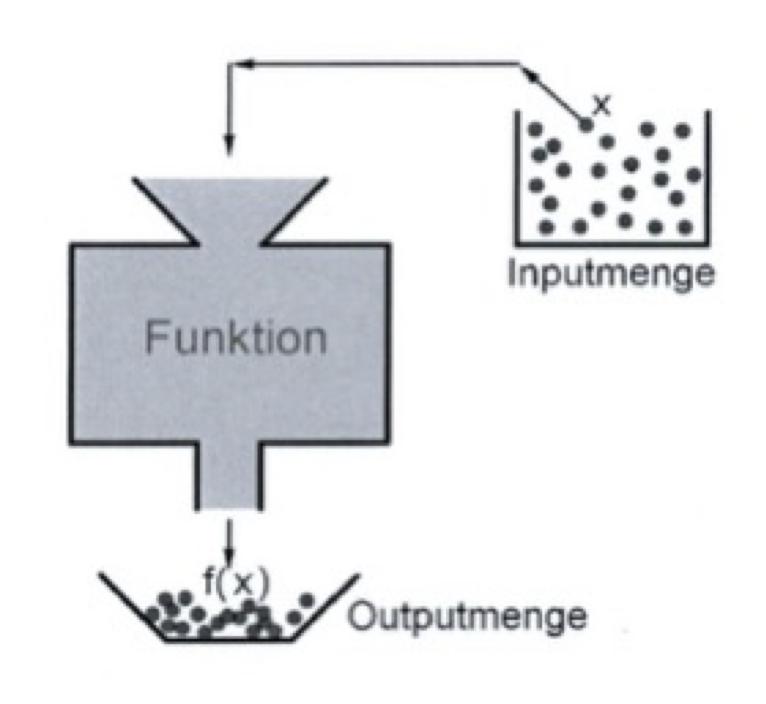
\includegraphics[width=\textwidth]{Einführung/im/Maschine.png}
\end{minipage}

\subsubsection{Funktion als Wolkendiagramm}
\begin{minipage}{0.6\textwidth}
    Ein anderes Bild, das man sich von einer Funktion machen kann, ist das rechts. Hier werden die beiden Mengen grafisch als Ovale stilisiert. Die Elemente der einzelnen Mengen werden als Punkte in den Ovalen dargestellt. Die Funktion ordnet jedem Punkt der Menge links einen Punkt der Menge rechts zu, was mit einem Pfeil dargestellt wird.
\end{minipage}
\begin{minipage}{0.4\textwidth}
    \begin{tikzpicture}[>={Stealth[length=10pt,width=8pt]},scale=0.8]
        % Mengen (hellgrau gefüllt)
        \fill[gray!15] (-2,0) circle (1.6);
        \fill[gray!15] (3.2,0) ellipse (1.3 and 2.0);

        % Ränder der Mengen
        \draw (-2,0) circle (1.6);
        \draw (3.2,0) ellipse (1.3 and 2.0);

        % Punkte x und y=f(x)
        \fill (-2.6,-0.4) circle (3pt) node[below] {$x$};
        \fill (4.0,0.3)  circle (3pt) node[below] {$y=f(x)$};

        \begin{scriptsize}
            % Abbildungspfeil mit grösserer Spitze
            \draw[<-,line width=1.2pt]
            (4.0,0.3) .. controls (1,1) .. (-2.6,-0.4)
            node[midway,above] {Funktion $f$};

            % Alternative (noch grössere Spitze):
            % \draw[->,thick,>=Stealth[scale=1.8]]
            % (-2.6,-0.4) .. controls (-0.5,-0.2) and (1.2,0.2) .. (4.0,0.3)
            % node[midway,above] {Funktion $f$};

            % Beschriftungen unter den Mengen
            \node at (-2,-1.95) {Definitionsmenge $D$};
            \node at (3.2,-2.25) {Wertemenge $W$};
        \end{scriptsize}
    \end{tikzpicture}
\end{minipage}
Die Eindeutigkeit (\glqq genau ein\grqq{})ist dann gegeben, wenn von jedem Punkt des Definitionsbereiches genau ein Pfeil abgeht. Umgekehrt dürfen aber mehrere Pfeile das gleiche Ziel haben:
\begin{center}
    \tikzset{
        dot/.style = {circle, inner sep=1.4pt, fill=black, draw=black},
        arr/.style = {->, >=Stealth, line width=1.5pt},
        setellipse/.style = {draw, ellipse, minimum width=30mm, minimum height=50mm}
    }
    \resizebox{\linewidth}{!}{%
        \begin{tikzpicture}[font=\small,>={Stealth[length=10pt,width=8pt]}]

            % ---------- Panel 1: eine Funktion ----------
            \begin{scope}
                \node[setellipse] (DL) at (0,0) {};
                \node[setellipse,right=32mm of DL] (WL) {};
                \node[above=2mm of DL] {Definitionsmenge};
                \node[above=2mm of WL] {Wertemenge};

                \node[dot] (a1) at ([xshift=-6mm,yshift=10mm]DL.center) {};
                \node[dot] (a2) at ([xshift=-6mm,yshift=0mm]DL.center) {};
                \node[dot] (a3) at ([xshift=-6mm,yshift=-10mm]DL.center) {};

                \node[dot] (b1) at ([xshift=6mm,yshift=12mm]WL.center) {};
                \node[dot] (b2) at ([xshift=6mm,yshift=0mm]WL.center) {};
                \node[dot] (b3) at ([xshift=6mm,yshift=-12mm]WL.center) {};

                \draw[arr] (a1) -- (b1);
                \draw[arr] (a2) -- (b3);
                \draw[arr] (a3) -- (b2);

                \node[below=6mm of $(DL.south)!0.5!(WL.south)$] {eine Funktion};
            \end{scope}

            % ---------- Panel 2: auch eine Funktion ----------
            \begin{scope}[xshift=10cm]
                \node[setellipse] (DM) at (0,0) {};
                \node[setellipse,right=32mm of DM] (WM) {};
                \node[above=2mm of DM] {Definitionsmenge};
                \node[above=2mm of WM] {Wertemenge};

                \node[dot] (c1) at ([xshift=-6mm,yshift=12mm]DM.center) {};
                \node[dot] (c2) at ([xshift=-6mm,yshift=2mm]DM.center) {};
                \node[dot] (c3) at ([xshift=-6mm,yshift=-8mm]DM.center) {};
                \node[dot] (d1) at ([xshift=6mm,yshift=0mm]WM.center) {};

                \draw[arr] (c1) -- (d1);
                \draw[arr] (c2) -- (d1);
                \draw[arr] (c3) -- (d1);

                \node[below=6mm of $(DM.south)!0.5!(WM.south)$] {auch eine Funktion};
            \end{scope}

            % ---------- Panel 3: keine Funktion ----------
            \begin{scope}[xshift=20cm]
                \node[setellipse] (DR) at (0,0) {};
                \node[setellipse,right=32mm of DR] (WR) {};
                \node[above=2mm of DR] {Definitionsmenge};
                \node[above=2mm of WR] {Wertemenge};

                \node[dot] (e1) at ([xshift=-6mm,yshift=10mm]DR.center) {};
                \node[dot] (e2) at ([xshift=-6mm,yshift=-4mm]DR.center) {};
                \node[dot] (f1) at ([xshift=6mm,yshift=12mm]WR.center) {};
                \node[dot] (f2) at ([xshift=6mm,yshift=-8mm]WR.center) {};
                \node[dot] (f3) at ([xshift=6mm,yshift=2mm]WR.center) {};

                % e1 hat zwei Bilder -> keine Funktion
                \draw[arr] (e1) .. controls +(1.4,0.8) .. (f1);
                \draw[arr] (e1) .. controls +(1.6,-0.2) .. (f3);
                \draw[arr] (e2) -- (f2);

                \node[below=6mm of $(DR.south)!0.5!(WR.south)$] {keine Funktion};
            \end{scope}

        \end{tikzpicture}}
\end{center}
$f(x)$ darf also nicht \glqq mehrere Ergebnisse\grqq{} haben.
\begin{example}
    Im Beispiel der Zuordnung \textit{Schüler} $\mapsto$ \textit{Gruppe} ist die Eindeutigkeit gegeben, da jeder Schüler genau einer Gruppe zugeordnet ist. Umgekehrt dürfen aber mehrere Schüler in die gleiche Gruppe eingeteilt werden (dies entspricht dem zweiten Bild oben, wo mehrere Pfeile auf das gleiche Ziel zeigen).
\end{example}

% \begin{example}
%     Die Definitionsmenge kann sich auch aus dem Sachzusammenhang ergeben. Falls wir pro Kilogramm Weltraum
% \end{example}
\subsection{Die Funktionsgleichung}
Im Gruppenbeispiel konnten wir die Zuordnung für jedes Element der Definitionsmenge explizit angeben.

In vielen Fällen ist dies aber nicht möglich, da die Definitionsmenge unendlich viele Elemente enthält. In solchen Fällen kann man eine \textbf{Funktionsgleichung} angeben, die beschreibt, wie der Output aus dem Input berechnet werden kann. Die Funktionsgleichung ist also quasi die Zuordnungsregel in Formelnform.

Im Beispiel der Einführungsaufabe 2. kann man eine Rechenanweisung angeben, mit der man ausgehend vom Input den Output berechnen kann:
\[f(x) =x^2\]
Will beispielsweise den Output an der Stelle $x=3$ bestimmen, kann man das $x$ in der Funktionsgleichung durch die $3$ ersetzen:
\[f(3)=3^2=9\]
Manchmal gibt es bei einer Funktionsgleichung auch unterschiedliche Rechenanweisungen, ja nachdem in welchem Bereich der Input liegt.

Dies ist zum Beispiel bei der Betragsfunktion der Fall. Anstatt mit $f(x)$ wird sie mit $|x|$ bezeichnet und ist folgendermassen definiert:
\[
    |x| = \begin{cases}
        x, \quad \text{falls } x \geq 0 \\
        -x, \quad \text{falls } x < 0
    \end{cases}
\]
$x=4$ wird auf $|4|=4$ abgebildet, $-5$ hingegen auf $|-5|=5$.
\subsection{Sprech- und Schreibweisen}
Der Begriff der Funktion ist über einen langen Zeitraum von etwa 150 Jahren entstanden. In dieser Zeit haben sich Mathematiker in verschiedenen Teilgebieten der Mathematik zwar intensiv mit Funktionen befasst, aber es gab noch keinen Überbegriff dafür. So sind unterschiedliche Sprechweisen entstanden, die das gleiche bedeuten und noch heute parallel verwendet werden:
\newcolumntype{L}[1]{>{\raggedright\arraybackslash}p{#1}}
\newcolumntype{C}[1]{>{\centering\arraybackslash}p{#1}}
\begin{table}[h]
    \centering
    \renewcommand{\arraystretch}{1.15} % etwas mehr Zeilenabstand
    \begin{tabular}{|L{0.3\linewidth}|L{0.3\linewidth}|L{0.3\linewidth}|}
        \hline
        \textit{Input} & \centering$\rightarrow$ & \textit{Output} \\
        \hline
        Argument       & Abbilden                & Funktionswert   \\
        Stelle         & Auswerten               & Wert            \\
        Urbild         &                         & Bild            \\
        $x$            &                         & $y$             \\
                       &                         & $f(x)$          \\
        \hline
    \end{tabular}
\end{table}

\begin{example}
    \begin{center}
        $f$ ordnet jeder Zahl ihr Quadrat zu.
    \end{center}
    Ausführlichste Variante:
    \[f: \R \to \R^+_0; \quad x \mapsto y = x^2\]
    Häufig interessiert man sich nicht so sehr für die beteiligten Mengen. Dann:
    \[f: x \mapsto y = x^2 \text{ oder } f: x \mapsto x^2\]
    Am meisten verwenden wir folgende Schreibweisen:
    \[y= x^2 \text{ oder } f(x) = x^2\]
\end{example}

\begin{example}
    \[f(x) = x^2\]
    \begin{itemize}
        \item $f(3)=9$ (sprich \glqq f von 3 ist 9\grqq{})
        \item \glqq Der Wert der Funktion f zum Argument 3 ist 9\grqq{}
        \item \glqq x=-3 wird auf y=9 abgebildet \grqq{}
        \item \glqq Der Funktionswert $9$ hat zwei Urbilder: $3$ und $-3$\grqq{}
        \item \glqq Das Bild von $-3$ unter der Funktion $f$ ist $9$\grqq{}
    \end{itemize}
\end{example}
\newpage

\subsection{Mehr zu Definitions- und Wertemengen}
In diesem Abschnitt werden wir uns mit den Mengen beschäftigen, die in der Definition einer Funktion vorkommen. Wir werden sehen, dass es zwei verschiedene Arten von Definitions- und Wertemengen gibt.
\subsubsection{Maximale Defintionsmenge}
% Die Definitionsmenge ist einfach die Menge aller für die Verarbeitung durch die Funktion zulässigen Werte. Dies kann ein Intervall oder eine komplizierter aufgebaute Menge sein.
Zu einer Funktion gehören die Definitionsmenge $\D$, die Wertemenge $\W$ und die Abbildungsvorschrift (meist in Form einer Funktionsgleichung). Oft ist die Definitionsmenge $\D$ nicht explizit angegeben. In diesem Fall ist die Definitionsmenge die grösstmögliche Menge an Eingabewerten, die man in die Funktionsgleichung einsetzen kann. Man spricht dann von der \textbf{maximalen} Definitionsmenge.
% \begin{example}
%     \[f(x) = x^2\]
%     Jede relle Zahl ist als Input erlaubt, deshalb ist $\D = \R$.

%     Es kann aber auch sein, dass wir nur an den Quadraten der positiven reellen Zahlen interessiert sind.
% \end{example}
\begin{deff}[Maximale Definitionsmenge]{}
    Die \textbf{maximale} Definitionsmenge einer Funktion ist die grösstmögliche Menge an Eingabewerten, für die die Funktion definiert ist.
\end{deff}

\begin{example}
    \[g(x) = \dfrac{1}{x}\]
    Die maximale Definitionsmenge ist $\D = \R \setminus \{0\}$, da die Funktion für $x=0$ nicht definiert ist.
\end{example}

\begin{example}
    \[h(x) = \sqrt{x}\]
    Die maximale Definitionsmenge ist $\D = \R_0^+$, da die Funktion für $x<0$ nicht definiert ist (die Wurzel aus einer negativen Zahl ist nicht definiert).
\end{example}

\begin{example}
    \[f(x)=10x +2\]
    Die maximale Definitionsmenge ist $\D = \R$, da jede reelle Zahl als Input erlaubt ist. Es kann allerdings Gründe geben nicht die gesamte Menge aller reellen Zahlen zu erlauben. Wenn beispielweise $f$ die Zuordnung \textit{Schrott in kg} $\mapsto$ \textit{Preis in CHF} beschreibt, dann ist die Definitionsmenge $\D = \R^+_0$, da negative Gewichte keinen Sinn ergeben. Ebenso könnte die Definitionsmenge aus anderen Gründen auch anders aussehen.
\end{example}
\subsubsection{Bildmenge}
Wie die Definitionsmenge gehört auch die Wertemenge zu einer Funktion. Die Wertemenge ist eine Menge, die alle möglichen Outputs enthält oder etwas genauer: Die Menge, in die die Funktion abbildet.
\begin{center}
    \tikzset{
        dot/.style = {circle, inner sep=1.4pt, fill=black, draw=black},
        arr/.style = {->, >=Stealth, line width=1.5pt},
        setellipse/.style = {draw, ellipse, minimum width=30mm, minimum height=50mm}
    }
    \resizebox{0.4\linewidth}{!}{%
        \begin{tikzpicture}[font=\small,>={Stealth[length=10pt,width=8pt]}]

            % ---------- Panel 1: eine Funktion ----------
            \begin{scope}
                \node[setellipse] (DL) at (0,0) {};
                \node[setellipse,right=32mm of DL] (WL) {};
                \node[above=2mm of DL] {$\D$};
                \node[above=2mm of WL] {$\W$};

                \node[dot] (a1) at ([xshift=-2mm,yshift=10mm]DL.center) {};
                \node[dot] (a2) at ([xshift=-2mm,yshift=0mm]DL.center) {};
                \node[dot] (a3) at ([xshift=-2mm,yshift=-10mm]DL.center) {};
                \node[dot] (a4) at ([xshift=-2mm,yshift=-20mm]DL.center) {};

                \node[dot] (b1) at ([xshift=2mm,yshift=18mm]WL.center) {};
                \node[dot] (b2) at ([xshift=2mm,yshift=6mm]WL.center) {};
                \node[dot] (b3) at ([xshift=2mm,yshift=-6mm]WL.center) {};
                \node[dot, red] (b4) at ([xshift=2mm,yshift=-18mm]WL.center) {};

                \draw[arr] (a1) -- (b1);
                \draw[arr] (a2) -- (b3);
                \draw[arr] (a3) -- (b2);
                \draw[arr] (a4) -- (b3);

                % \node[below=6mm of $(DL.south)!0.5!(WL.south)$] {eine Funktion};
            \end{scope}
        \end{tikzpicture}}
\end{center}
Hier werden nicht alle Werte in $\W$ getroffen (der rote Wert). Dies ist erlaubt, genauso gut könnte man aber auch als Wertemenge nur die Werte angeben, die tatsächlich getroffen werden.
\begin{deff}[Bildmenge]{}
    Die \textbf{Bildmenge} einer Funktion $f$ ist die Menge aller Werte, die tatsächlich getroffen werden. Sie ist also eine Teilmenge der Wertemenge $\W$.
\end{deff}
Oft gibt man für die Wertemenge einfach $\R$ an, da die Outputs jeder Funktion, die uns begegnet, alle in $\R$ liegen. Manchmal will man es aber genauer wissen und gibt die Bildmenge an.
\begin{example}
    \[f(x) = x^2\]
    Als Wertemenge kann man $\W = \R$ angeben, da das Quadrat jeder reellen Zahl eine reelle Zahl ergibt. Die Bildmenge ist aber \(\mathbb{R}_0^+\), da nur nichtnegative Zahlen getroffen werden und gleichzeitig jede nichtnegative reelle Zahl als Funktionswert vorkommt. Es sind also folgende Wertemengen möglich:
    \begin{itemize}
        \item $\W = \R$
        \item $\W = \R_0^+$
        \item $\W = [-10, \infty [$
    \end{itemize}
    $[1,2]$ könnte man nicht als Wertemenge angeben, da sonst für beispielsweise $x=3$ der Output $y=9$ nicht in der Wertemenge liegt.
\end{example}
\newpage
\subsubsection{Urbild bestimmen}
Das Urbild eines Funktionswertes (Outputs) $y$ unter einer Funktion $f$ ist die Menge aller Werte $x$, die auf $y$ abgebildet werden.
\begin{example}
    \[f(x) = x^2-5x + 8\]
    Bestimmen Sie das Urbild von $y=2$ unter $f$.

    \kariert{10}
\end{example}
\newpage
\subsubsection{Übungen}
\begin{enumerate}
    \item Welche Zuordnung stellt eine Funktion dar?
          \begin{multicols}{4}
              \begin{enumerate}[label=\roman*)]
                  \tikzset{
                      dot/.style = {circle, inner sep=2.5pt, fill=black, draw=black},
                      arr/.style = {->, >=Stealth, line width=1.5pt},
                      setellipse/.style = {draw, ellipse, minimum width=30mm, minimum height=50mm}
                  }
                  \item \resizebox{\linewidth}{!}{%
                            \begin{tikzpicture}[font=\small, >={Stealth[length=10pt,width=8pt]}]
                                \node[setellipse] (DL) at (0,0) {};
                                \node[setellipse, right=10mm of DL] (WL) {};

                                \node[dot] (a1) at ([yshift=5mm]DL.center) {};
                                \node[dot] (a2) at ([yshift=-5mm]DL.center) {};

                                \node[dot] (b1) at ([yshift=12mm]WL.center) {};
                                \node[dot] (b2) at ([yshift=0mm]WL.center) {};
                                \node[dot] (b3) at ([yshift=-12mm]WL.center) {};

                                \draw[arr] (a1) -- (b1);
                                \draw[arr] (a2) -- (b3);
                            \end{tikzpicture}%
                        }
                  \item \resizebox{\linewidth}{!}{%
                            \begin{tikzpicture}[font=\small, >={Stealth[length=10pt,width=8pt]}]
                                \node[setellipse] (DL) at (0,0) {};
                                \node[setellipse, right=10mm of DL] (WL) {};

                                \node[dot] (a1) at ([yshift=10mm]DL.center) {};
                                \node[dot] (a2) at ([yshift=0mm]DL.center) {};
                                \node[dot] (a3) at ([yshift=-10mm]DL.center) {};

                                \node[dot] (b1) at ([yshift=5mm]WL.center) {};
                                \node[dot] (b2) at ([yshift=-5mm]WL.center) {};

                                \draw[arr] (a1) -- (b1);
                                \draw[arr] (a3) -- (b2);
                            \end{tikzpicture}%
                        }
                  \item \resizebox{\linewidth}{!}{%
                            \begin{tikzpicture}[font=\small, >={Stealth[length=10pt,width=8pt]}]
                                \node[setellipse] (DL) at (0,0) {};
                                \node[setellipse, right=10mm of DL] (WL) {};

                                \node[dot] (a1) at ([yshift=10mm]DL.center) {};
                                \node[dot] (a2) at ([yshift=0mm]DL.center) {};
                                \node[dot] (a3) at ([yshift=-10mm]DL.center) {};

                                \node[dot] (b1) at ([yshift=10mm]WL.center) {};
                                \node[dot] (b2) at ([yshift=0mm]WL.center) {};
                                \node[dot] (b3) at ([yshift=-10mm]WL.center) {};

                                \draw[arr] (a1) -- (b1);
                                \draw[arr] (a3) -- (b1);
                                \draw[arr] (a3) -- (b2);
                                \draw[arr] (a3) -- (b3);
                            \end{tikzpicture}%
                        }
                  \item \resizebox{\linewidth}{!}{%
                            \begin{tikzpicture}[font=\small, >={Stealth[length=10pt,width=8pt]}]
                                \node[setellipse] (DL) at (0,0) {};
                                \node[setellipse, right=10mm of DL] (WL) {};

                                \node[dot] (a1) at ([yshift=12mm]DL.center) {};
                                \node[dot] (a2) at ([yshift=4mm]DL.center) {};
                                \node[dot] (a3) at ([yshift=-4mm]DL.center) {};
                                \node[dot] (a4) at ([yshift=-12mm]DL.center) {};

                                \node[dot] (b1) at ([yshift=10mm]WL.center) {};
                                \node[dot] (b2) at ([yshift=0mm]WL.center) {};
                                \node[dot] (b3) at ([yshift=-10mm]WL.center) {};

                                \draw[arr] (a1) -- (b1);
                                \draw[arr] (a2) -- (b2);
                                \draw[arr] (a3) -- (b3);
                                \draw[arr] (a4) -- (b3);
                            \end{tikzpicture}%
                        }
              \end{enumerate}
          \end{multicols}
    \item Entscheiden Sie, ob die Zuordnung eindeutig und damit eine Funktion ist.
          \begin{enumerate}
              \item Person $\mapsto$ Geburtsdatum
              \item AHV-Nummer $\mapsto$ Person
              \item Person in der Schweiz $\mapsto$ Festnetztelefonnummer
              \item Körpergrösse einer Person $\mapsto$ Alter der Person
              \item Alter einer Person $\mapsto$ Körpergrösse der Person
              \item Höhe in m ü. M. an einem Ort $\mapsto$ Luftdruck in dieser Höhe an diesem Ort
              \item Tageslänge $\mapsto$ Tag im Jahr
          \end{enumerate}
    \item An einer Skiliftstation wurde an einem Wintertag zu jeder Stunde die Temperatur in $^\circ$C gemessen und protokolliert.
          Entscheiden Sie aufgrund der Wertetabelle, ob es sich bei den Zuordnungen $U \mapsto T$ bzw. $T \mapsto U$ um eine Funktion handelt oder nicht. Begründen Sie Ihre Antwort.
          \begin{center}
              \begin{tabular}{c|cccccccccc}
                  Uhrzeit $U$    & 8    & 9  & 10 & 11 & 12 & 13 & 14  & 15 & 16 & 17 \\
                  \hline
                  Temperatur $T$ & -4.5 & -4 & -2 & -1 & 0  & 1  & 0.5 & 1  & -1 & -3
              \end{tabular}
          \end{center}
    \item Entscheiden Sie, ob es sich bei der Zuordnung um eine Funktion handelt oder nicht. Falls ja, geben Sie die Funktionsgleichung inklusive Definitionsbereich an.
          \begin{enumerate}
              \item Jeder ganzen Zahl wird ihr Quadrat zugeordnet.
              \item Jeder natürlichen Zahl wird die um 2 grössere Zahl zugeordnet.
              \item Jeder negativen Zahl wird ihr Betrag zugeordnet.
              \item Der Quersumme einer natürlichen Zahl $n$ wird die Zahl $n$ zugeordnet.
              \item Jeder reellen Zahl ausser $0$ wird ihr Kehrwert zugeordnet.
              \item Jeder positiven reellen Zahl $x$ wird diejenige Zahl zugeordnet, deren Quadrat $x$ ergibt.
          \end{enumerate}
          % \item Entscheiden Sie, ob die Zuordnung eine Funktion ist oder nicht.
          %       \begin{enumerate}
          %           \item Jeder natürlichen Zahl wird ihre Anzahl Teiler zugeordnet.
          %           \item \( x \in \{2,3,4\} \mapsto \) natürliche Zahl \( n \) zwischen 1 und 11, die den Teiler \( x \) hat.
          %           \item \( f : x \mapsto y = 2 \cdot x \)
          %           \item \( f : x \mapsto y = -x \)
          %       \end{enumerate}
    \item Gegeben ist die Funktion \( g \) mit der Funktionsgleichung
          \[
              g(x) = 2x^2 - x.
          \]
          Berechnen Sie den gesuchten Funktionswert \( g(x) \).
          \begin{multicols}{4}
              \begin{enumerate}
                  \item \( g(-2) \)
                  \item \( g(0) \)
                  \item \( g\left(\tfrac{1}{2}\right) \)
              \end{enumerate}
          \end{multicols}
    \item Gegeben ist die Funktion \( f(x) = \dfrac{6}{x - 1} \)
          \begin{enumerate}[label=\alph*)]
              \item Berechnen Sie \( f(0) \).
              \item Berechnen Sie den Funktionswert an der Stelle 3.
              \item Geben Sie das Urbild von 12 an.
              \item Geben Sie den grösstmöglichen Definitionsbereich und eine mögliche Wertemenge an.
              \item Welche Argumente werden auf sich \underline{selber} abgebildet? (Tipp: Produkt = 0)
          \end{enumerate}

    \item \label{aufgabe:vorzeichenfunktion}Die Vorzeichenfunktion \( \operatorname{sgn}(x) \) ist wie folgt definiert:
          \[
              \operatorname{sgn}(x) =
              \begin{cases}
                  1,  & \text{falls } x > 0, \\
                  0,  & \text{falls } x = 0, \\
                  -1, & \text{falls } x < 0
              \end{cases}
          \]
          \begin{enumerate}[label=\alph*)]
              \item Bestimmen Sie \( \operatorname{sgn}(\pi) \) und \( \operatorname{sgn}(-100) \).
              \item Geben Sie den maximalen Definitionsbereich und die Bildmenge der Vorzeichenfunktion an.
              \item Sei \( a \) eine beliebige reelle Zahl. Was ist dann \( |a| \cdot \operatorname{sgn}(a) \)?
                    \begin{enumerate}[label=\roman*)]
                        \item Falls \( a > 0 \) ist? \\
                        \item Falls \( a = 0 \) ist? \\
                        \item Falls \( a < 0 \) ist?
                    \end{enumerate}
          \end{enumerate}

    \item Sei \( p: x \mapsto 2x + 1 \)
          \begin{enumerate}[label=\alph*)]
              \item Geben Sie den maximalen Definitionsbereich und die Bildmenge der Funktion \( p \) an.
              \item Berechnen Sie \( p(3) \).
              \item Berechnen Sie \( p(p(3)) \). Wobei das so zu verstehen ist, dass der Output \( p(3) \) nochmals als Input der Funktion \( p \) dient.
              \item Was ist dann \( p(p(p(3))) \)?
              \item Was ist das Urbild von \( 7 \) unter \( p \)?
              \item Welches Argument wird auf sich selbst abgebildet?
          \end{enumerate}

    \item Betrachten Sie die Wurzelfunktion \( y = \sqrt{x} \). Der Output dieser Funktion ist die nicht-negative Zahl \( y \) mit \( y^2 = x \). Zum Beispiel \( \sqrt{9} = 3 \).
          \begin{enumerate}[label=\alph*)]
              \item Was ist \( \sqrt{36} \)? Und was \( \sqrt{0} \)?
              \item Wieso muss betont werden, dass \( y \) nicht negativ ist?
              \item Geben Sie den maximalen Definitionsbereich und die Bildmenge der Wurzelfunktion an.
              \item Bestimmen Sie das Urbild von \(7\) unter der Wurzelfunktion.
              \item Gibt es Argumente, die kleiner sind als deren Funktionswerte? Welche?
          \end{enumerate}




    \item \textbf{Challenge:} \\
          Betrachten Sie die Mengen \( A = \{1, 2, 3, 4\} \) und \( B = \{1, 2, 3, 4, 5, 6\} \).
          Sei \( f \) eine Funktion, deren Definitionsbereich \( A \) ist und deren Wertemenge eine Teilmenge von \( B \) ist.
          \begin{enumerate}[label=\alph*)]
              \item Wie viele solche Funktionen gibt es?
              \item Wie viele solche Funktionen gibt es, bei denen kein Element auf sich selbst abgebildet wird?
          \end{enumerate}

          % \item \label{aufgabe:teileranzahlfunktion} \textbf{Challenge:} \\
          %       Für die Teileranzahl-Funktion \[ \tau(n)= \textit{Anzahl Teiler von n}\] kann nicht so leicht eine Funktionsgleichung angeben. Allerdings kann man \( \tau(n) \) aus der Primfaktorzerlegung von \( n \) bestimmen:
          %       \[
          %           \text{Sei } n = p_1^{a_1} \cdot p_2^{a_2} \cdots p_k^{a_k}
          %       \]
          %       die Primfaktorzerlegung von \( n \). Berechnen Sie daraus \( \tau(n) \).
\end{enumerate}
\newpage
\subsubsection{Lösungen}

\begin{enumerate}

    \item
          \begin{multicols}{4}
              \begin{enumerate}
                  \item ja
                  \item nein
                  \item nein
                  \item ja
              \end{enumerate}
          \end{multicols}

    \item
          \begin{multicols}{3}
              \begin{enumerate}
                  \item Funktion
                  \item Funktion
                  \item keine Funktion
                  \item keine Funktion
                  \item keine Funktion % NEU/KORRIGIERT
                  \item Funktion
                  \item keine Funktion % NEU/KORRIGIERT
              \end{enumerate}
          \end{multicols}

    \item
          $U \mapsto T$: Funktion;
          $T \mapsto U$: keine Funktion, da beispielsweise für $T=1$
          zwei unterschiedliche Uhrzeiten zugeordnet sind.

    \item
          \begin{enumerate}
              \item Funktion: $f(x)=x^2$, $D=\mathbb{Z}$ % NEU/KORRIGIERT

              \item Funktion: $f(x)=x+2$, $D=\mathbb{N}$ % NEU/KORRIGIERT

              \item Funktion: $f(x)=|x|$, $D=\mathbb{R}^-$ % NEU/KORRIGIERT

              \item keine Funktion % NEU/KORRIGIERT

              \item Funktion: $f(x)=\dfrac{1}{x}$,
                    $D=\mathbb{R}\setminus\{0\}$ % NEU/KORRIGIERT

              \item keine Funktion, da für jede Zahl zwei verschiedene Werte zugeordnet wären  (Bsp.: für $x=1$ wäre $y=-1$ und $y=1$ möglich) % NEU/KORRIGIERT
          \end{enumerate}

    \item
          \begin{multicols}{4}
              \begin{enumerate}
                  \item $g(-2)=10$
                  \item $g(0)=0$
                  \item $g\left(\tfrac12\right)=0$
              \end{enumerate}
          \end{multicols}

    \item
          $f(x)=\dfrac{6}{x-1}$

          \begin{enumerate}
              \item $f(0)=-6$

              \item $f(3)=3$

              \item $x=\dfrac{3}{2}$

              \item $D=\mathbb{R}\setminus\{1\};
                        \quad W=\mathbb{R}\setminus\{0\}$

              \item
                    $\dfrac{6}{x-1}=x
                        \Leftrightarrow x^2-x-6=0
                        \Leftrightarrow (x-3)(x+2)=0
                        \Leftrightarrow x=3 \text{ oder } x=-2$
          \end{enumerate}

    \item Vorzeichenfunktion

          \begin{enumerate}
              \item $\operatorname{sgn}(\pi)=1$ und
                    $\operatorname{sgn}(-100)=-1$

              \item $D=\mathbb{R};
                        \quad W=\{-1,0,1\}$

              \item $|a|\cdot\operatorname{sgn}(a)=a$
          \end{enumerate}

    \item
          $p:x\mapsto 2x+1$

          \begin{enumerate}
              \item $D=\mathbb{R};
                        \quad W=\mathbb{R}$ % NEU/KORRIGIERT

              \item $p(3)=7$

              \item $p(p(3))=15$

              \item $p(p(p(3)))=31$

              \item $x=3$ % NEU/KORRIGIERT

              \item $x=-1$ % NEU/KORRIGIERT
          \end{enumerate}

    \item Wurzelfunktion

          \begin{enumerate}
              \item $\sqrt{36}=6$ und $\sqrt{0}=0$

              \item Weil es sonst zu einem Input zwei Outputs geben könnte;
                    dann wäre es keine Funktion mehr; Beispiel: für $y^2=9$ kommen zwei mögliche Outputs in Frage: $y=3$ und $y=-3$.

              \item $D=\mathbb{R}_0^+;
                        \quad W=\mathbb{R}_0^+$

              \item $x=49$ % NEU/KORRIGIERT

              \item Ja, alle $x\in]0,1[$.
          \end{enumerate}

    \item Challenge:

          \begin{enumerate}
              \item $1296$
              \item $625$
          \end{enumerate}

\end{enumerate}
\newpage

\section{Graphen von Funktionen}
\subsection{Einführungsaufgabe}
\begin{center}
    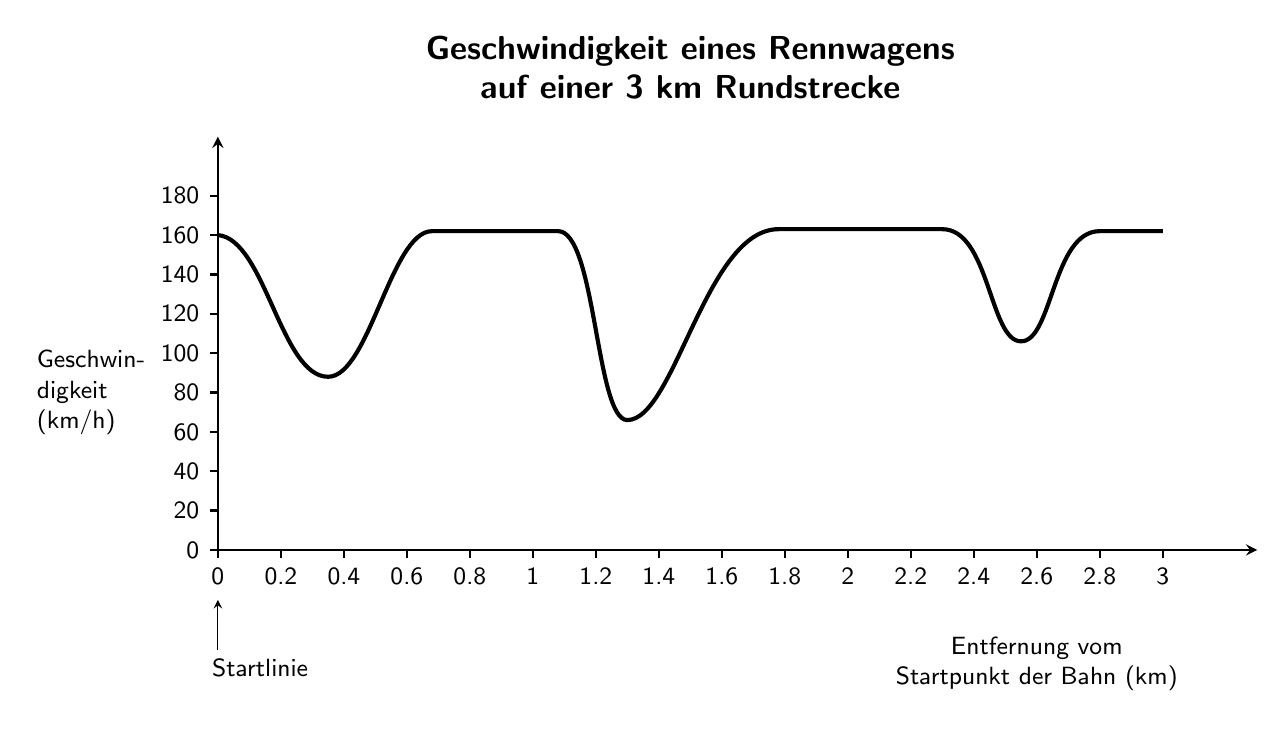
\begin{tikzpicture}[x=4cm, y=0.025cm, >=stealth, font=\sffamily\small]
        % Achsen
        \draw[thick,->] (0,0) -- (3.3,0);
        \draw[thick,->] (0,0) -- (0,210);

        % x-Achse: Ticks und Beschriftung unten
        \foreach \x in {0,0.2,0.4,0.6,0.8,1,1.2,1.4,1.6,1.8,2,2.2,2.4,2.6,2.8,3}
        \draw[thick] (\x,0) -- ++(0,-3pt) node[below] {\x};
        % x-Achse: Zwischenwerte oben
        % \foreach \x in {0.5,1.5,2.5}
        % \draw[thick] (\x,0) -- ++(0,-3pt) node[above=4pt] {\x};

        % y-Achse
        \foreach \y in {0,20,...,180}
        \draw[thick] (0,\y) -- ++(-3pt,0) node[left] {\y};

        % Geschwindigkeitskurve
        \draw[line width=1.5pt]
        (0,160)
        .. controls (0.15,158) and (0.20,88)  .. (0.35,88)
        .. controls (0.48,88)  and (0.55,162) .. (0.68,162)
        -- (1.08,162)
        .. controls (1.20,162) and (1.20,66)  .. (1.30,66)
        .. controls (1.45,66)  and (1.55,163) .. (1.78,163)
        -- (2.30,163)
        .. controls (2.45,163) and (2.45,106) .. (2.55,106)
        .. controls (2.65,106) and (2.65,162) .. (2.80,162)
        -- (3,162);

        % Beschriftungen
        \node[align=center, font=\sffamily\bfseries\large] at (1.5,245)
        {Geschwindigkeit eines Rennwagens\\auf einer 3 km Rundstrecke};
        \node[align=left, anchor=east] at (-0.2,80)
        {Geschwin-\\digkeit\\(km/h)};
        \node[align=center, anchor=north] at (2.6,-28pt)
        {Entfernung vom\\Startpunkt der Bahn (km)};
        \draw[->] (0,-36pt) -- (0,-18pt);
        \node[anchor=north west, inner xsep=0pt] at (-0.02,-36pt) {Startlinie};
    \end{tikzpicture}
\end{center}
Das Bild oben zeigt den Verlauf der Funktion, die jeder Stelle der 3km langen Rennstrecke die Geschwindigkeit des Rennwagens zuordnet.
\begin{enumerate}
    \item Wo auf der Strecke ist die Geschwindigkeit am niedrigsten?
    \item Was ist die maximale Geschwindigkeit des Rennwagens?
    \item Welche der unten abgebildeten Rennstrecken passt zum Geschwindigkeitsprofil oben? Wieso?
\end{enumerate}
\begin{center}
    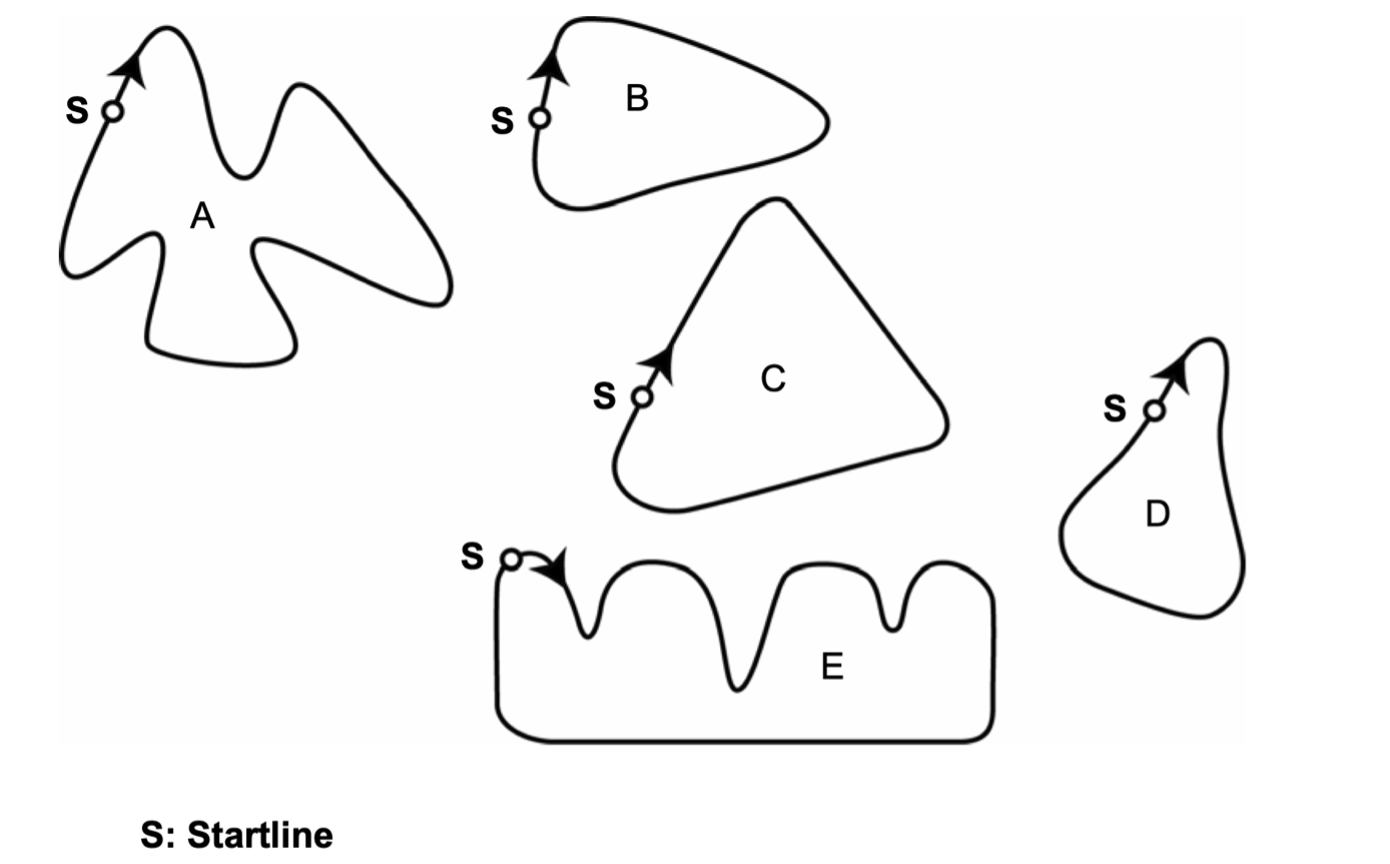
\includegraphics[width=0.6\textwidth]{Einführung/im/Rennstrecken.png}
\end{center}
\begin{enumerate}
    \setcounter{enumi}{3}
    \item Im obigen Diagramm ist eine Zuordnung/Funktion dargestellt. Welche beiden Grössen werden im obigen Diagramm einander zugeordnet?
    \item Geben Sie ein paar Funktionswerte (ungefähr) an, die Sie aus dem Diagramm ablesen können.
    \item Geben Sie den Definitions- und Wertebereich der Funktion an.
\end{enumerate}
\newpage
\subsection{Das kartesische Koordinatensystem und der Graph einer Funktion}
Was für zahlreiche Alltagssituationen zutrifft, stimmt auch für Funktionen: Ein Bild sagt mehr als tausend Worte. Schafft man es, eine Funktion bildlich darzustellen, so werden ihre Besonderheiten auf einen Blick sichtbar.

Um Funktionen zu visualisieren, verwendet man in der Regel ein Kartesisches  Koordinatensystem.
\begin{center}
    \begin{tikzpicture}[scale=1.0, >=stealth]

        % Achsen zeichnen
        \draw[->] (-4.5,0) -- (4.5,0) node[right] {Abszisse};
        \draw[->] (0,-3.5) -- (0,3.5) node[above] {Ordinate};

        % Quadranten beschriften
        \node at (2,2) {1.~Quadrant};
        \node at (-2,2) {2.~Quadrant};
        \node at (-2,-2) {3.~Quadrant};
        \node at (2,-2) {4.~Quadrant};

        % Achsenbeschriftungen (x und y)
        \node at (4.3,0.3) {$x$};
        \node at (0.3,3.3) {$y$};

        % Ticks für x-Achse
        \foreach \x in {-4,-3,-2,-1,1,2,3,4}
        \draw (\x,0.1) -- (\x,-0.1) node[below=4pt] {\x};

        % Ticks für y-Achse
        \foreach \y in {-3,-2,-1,1,2,3}
        \draw (0.1,\y) -- (-0.1,\y) node[left=4pt] {\y};

    \end{tikzpicture}
\end{center}
Der Graph einer Funktion ist eine Menge von Punkten im Kartesischen Koordinatensystem:
\begin{center}
    \begin{tikzpicture}
        \begin{axis}[
                axis lines=middle,
                axis line style={->},
                xlabel={$x$},
                ylabel={$y$},
                xmin=-4.5, xmax=4.5,
                ymin=-20, ymax=30,
                xtick distance=1,
                ytick distance=10,
                enlargelimits=false,
                clip=false,
                width=0.8\textwidth
            ]

            % Beispielfunktion (kubisch), so dass f(2) ≈ -6.33
            \addplot[
                domain=-4.3:3.5, samples=200, smooth,
                thick, green!60!black
            ]
            {16/3/22.1*(x+4.2)*(x)*x*(x-2.9)};

            % Markierter Punkt (2, -5.33)
            \addplot[only marks, mark=*, mark size=2.2pt, blue]
            coordinates {(2, -5.33)};
            % Beschriftung unterhalb des Punktes
            \node[blue, below] at (axis cs:2,-5.33) {(2,\,-5.33)};

            % Hilfslinien: x = 2 (vertikal) und y = -16/3 (horizontal)
            \addplot[dashed] coordinates {(2,0) (2,-5.33)};
            \addplot[dashed] coordinates {(0,-16/3) (2,-16/3)};

            % Achsenbeschriftungen an den Hilfslinien
            % \node[anchor=north] at (axis cs:2,0) {$2$};
            \node[anchor=east]  at (axis cs:0,-16/3) {$-\dfrac{16}{3}$};

        \end{axis}
    \end{tikzpicture}
\end{center}
\begin{itemize}
    \item Der Punkt $(2,-\frac{16}{3})$ liegt auf dem Graphen von $f$, weil $f(2)=-\frac{16}{3}$
    \item Auf der x-Achse sind die Input-Werte (Argumente) der Funktion abgetragen, auf der y-Achse die Output-Werte (Funktionswerte).
    \item Im Bereich $[-4,4]$ ist der kleinste Funktionswert für $x=-3$ erreicht und ist ungefährt $y=-15$
\end{itemize}
\begin{deff}[Graph einer Funktion]{}
    Der Graph einer Funktion $f$ ist die Menge der Punkte mit den Koordinaten $(x,y)$ im Kartesischen Koordinatensystem mit der Eigenschaft, dass $y$ der Output der Funktion zum Input $x$ ist:
    \[\operatorname{Graph} f=\{(x,y)| y=f(x)\}\]
\end{deff}

\subsection{Nicht jede Kurve ist der Graph einer Funktion}
Wichtige Eigenschaft einer Funktion:
\begin{center}
    \textbf{Zuordnung muss eindeutig sein} oder \textbf{Pro Input genau ein Output}
\end{center}
Übertragen auf den Funktionsgraphen:
\begin{center}
    \textbf{Keine zwei Graphenpunkten mit derselben x-Koordinate}
\end{center}
\begin{example}
    \begin{minipage}{0.5\textwidth}
        \begin{center}
            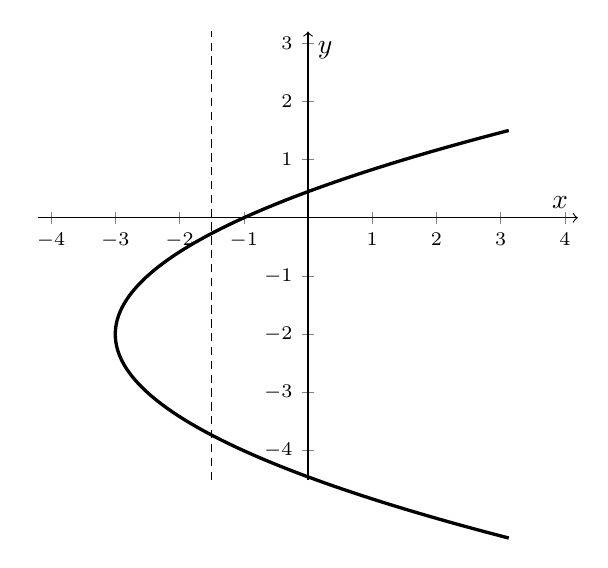
\begin{tikzpicture}
                \begin{axis}[
                        axis lines=middle,
                        axis line style={->},
                        xlabel={$x$},
                        ylabel={$y$},
                        xmin=-4.2, xmax=4.2,
                        ymin=-4.5, ymax=3.2,
                        xtick distance=1,
                        ytick distance=1,
                        enlargelimits=false,
                        clip=false,
                        tick label style={font=\scriptsize}
                    ]

                    % vertikale gestrichelte Linie bei x = -2
                    \addplot[densely dashed] coordinates {(-1.5,-4.5) (-1.5,3.2)};

                    % parametrische Kurve: x(t) = t^2 - 2, y(t) = t^3 - t
                    \addplot[
                        domain=-0.5:6.5,
                        samples=400,
                        smooth,
                        very thick
                    ] ({0.5*(x-3)^2-3},{x-5});

                \end{axis}
            \end{tikzpicture}
        \end{center}
    \end{minipage}
    \begin{minipage}{0.5\textwidth}
        Die Kurve in der Grafik rechts kann nicht der Graph einer Funktion sein, weil die Parallele zur y-Achse an der Stelle $x=-1.6$ die Kurve in zwei Punkten schneidet. Das würde bedeuten, dass die entsprechende Zuordnung für den Input $x=-1.6$ zwei mögliche Outputs liefert. (ungefähr $-0.4$ und $-4$). Das widerspricht der Vorgabe, dass die Funktion eindeutig sein muss.
    \end{minipage}
\end{example}
\newpage
\subsection{Von der Funktiongleichung zum Funktionsgraphen}
\[g(x)=2x-x^2\]
Um den Graph einer Funktion zu zeichnen, erstellt man zuerst eine sogenannte Wertetabelle. Darin werden die Funktionswerte an einigen Stellen eingetragen. Für das vorliegende Beispiel wurden die Werte für ganzzahlige Argumente zwischen $-3$ und $5$ berechnet:
\begin{center}
    \newcolumntype{Y}{>{\centering\arraybackslash}X}

    \begin{tabularx}{\linewidth}{|>{\centering\arraybackslash}m{2cm}|*{9}{Y|}}
        \hline
        $x$      & $-3$  & $-2$ & $-1$ & $0$ & $1$ & $2$ & $3$  & $4$  & $5$   \\
        \hline
        $y=g(x)$ & $-15$ & $-8$ & $-3$ & $0$ & $1$ & $0$ & $-3$ & $-8$ & $-15$ \\
        \hline
    \end{tabularx}
\end{center}
Anhand der Wertetabelle erkennt man, dass für die vorliegende Funktion ein Koordinatensystem nötig ist, auf welchem die x-Achse im Bereich -3 bis 5 abgebildet ist, während die y-Werte zwischen -15  und 1 liegen:
\begin{center}
    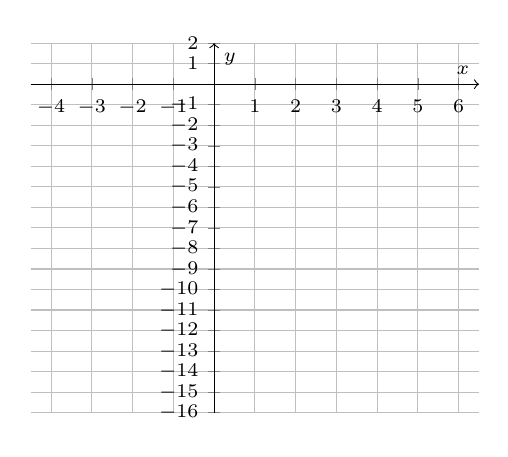
\begin{tikzpicture}
        \begin{axis}[
                axis lines=middle,
                axis line style={->},
                % axis equal image,
                xlabel={$x$},
                ylabel={$y$},
                xmin=-4.5, xmax=6.5,
                ymin=-16, ymax=2,
                xtick distance=1,
                ytick distance=1,
                grid=both,
                enlargelimits=false,
                clip=false,
                width=0.6\textwidth,
                font=\scriptsize,
            ]
        \end{axis}
    \end{tikzpicture}
\end{center}
Jedes Zahlenpärchen $(x,y)$ in der Wertetabelle entspricht einem Punkt auf dem Graphen:
\begin{center}
    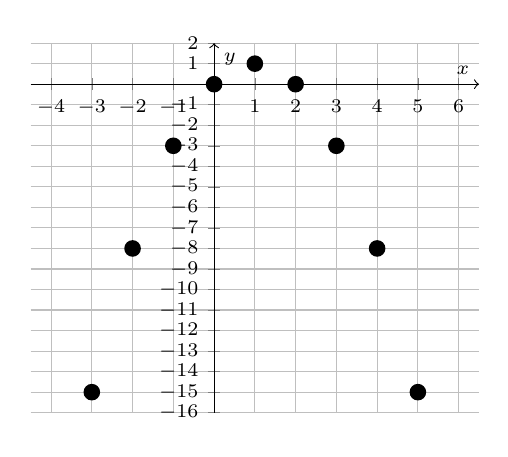
\begin{tikzpicture}
        \begin{axis}[
                axis lines=middle,
                axis line style={->},
                % axis equal image,
                xlabel={$x$},
                ylabel={$y$},
                xmin=-4.5, xmax=6.5,
                ymin=-16, ymax=2,
                xtick distance=1,
                ytick distance=1,
                grid=both,
                enlargelimits=false,
                clip=false,
                width=0.6\textwidth,
                font=\scriptsize,
            ]
            \fill (-3,-15) circle (3pt);
            \fill (-2,-8)  circle (3pt);
            \fill (-1,-3)  circle (3pt);
            \fill ( 0, 0)  circle (3pt);
            \fill ( 1, 1)  circle (3pt);
            \fill ( 2, 0)  circle (3pt);
            \fill ( 3,-3)  circle (3pt);
            \fill ( 4,-8)  circle (3pt);
            \fill ( 5,-15) circle (3pt);
        \end{axis}
    \end{tikzpicture}
\end{center}
Da der Definitionsbereich von $g$ alle reellen Zahlen umfasst, ist diese Menge von einzelnen Punkten nur einen kleinen Ausschnitt des Graphen. Den Verlauf zwischen den Punkten wird geschätzt, indem man die Punkte durch eine \glqq glatte\grqq{} Kurve verbindet. Ist man sich unsicher, können auch noch zusätzliche Werte berechnet werden, wie z.B. $f(\frac{1}{2})=\frac{3}{4}$.
\begin{center}
    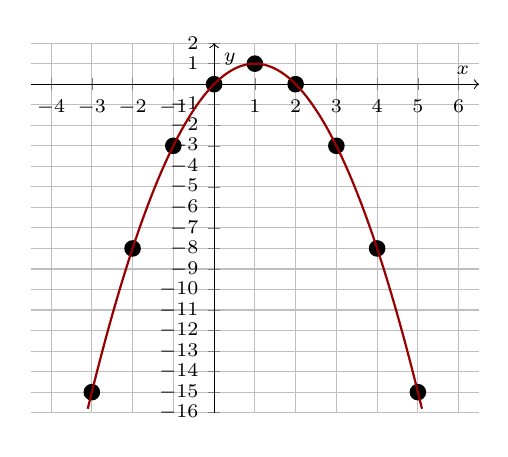
\begin{tikzpicture}
        \begin{axis}[
                axis lines=middle,
                axis line style={->},
                % axis equal image,
                xlabel={$x$},
                ylabel={$y$},
                xmin=-4.5, xmax=6.5,
                ymin=-16, ymax=2,
                xtick distance=1,
                ytick distance=1,
                grid=both,
                enlargelimits=false,
                clip=false,
                width=0.6\textwidth,
                font=\scriptsize,
            ]
            \fill (-3,-15) circle (3pt);
            \fill (-2,-8)  circle (3pt);
            \fill (-1,-3)  circle (3pt);
            \fill ( 0, 0)  circle (3pt);
            \fill ( 1, 1)  circle (3pt);
            \fill ( 2, 0)  circle (3pt);
            \fill ( 3,-3)  circle (3pt);
            \fill ( 4,-8)  circle (3pt);
            \fill ( 5,-15) circle (3pt);
            \addplot[
                domain=-3.1:5.1, samples=200, smooth,
                thick, red!60!black
            ]
            {2*x-x^2};
        \end{axis}
    \end{tikzpicture}
\end{center}
\newpage
\subsection{Übungen}
\begin{enumerate}
    \item Welche Kurve ist der Graph einer Funktion $x \mapsto y$?
          \begin{multicols}{4}
              \begin{enumerate}[label=\roman*)]
                  \item 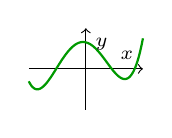
\begin{tikzpicture}
                            \begin{axis}[
                                    axis lines=middle,
                                    axis line style={->},
                                    xlabel={$x$},
                                    ylabel={$y$},
                                    label style={font=\scriptsize},
                                    xmin=-11, xmax=11,
                                    ymin=-20, ymax=20,
                                    xtick distance=1,
                                    ytick distance=20,
                                    enlargelimits=false,
                                    clip=false,
                                    width=0.25\textwidth,
                                    xtick=\empty,        % keine x-Ticks
                                    ytick=\empty,
                                ]

                                % Beispielfunktion (kubisch), so dass f(2) ≈ -6.33
                                \addplot[
                                    domain=-11:11, samples=100, smooth,
                                    thick, green!60!black
                                ]
                                {16/3/52.1*(x+11.2)*(x+7)*(1/5*(x+7)-2.9)^2-5};
                            \end{axis}
                        \end{tikzpicture}
                  \item 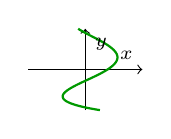
\begin{tikzpicture}
                            \begin{axis}[
                                    axis lines=middle,
                                    axis line style={->},
                                    xlabel={$x$},
                                    ylabel={$y$},
                                    label style={font=\scriptsize},
                                    xmin=-20, xmax=20,
                                    ymin=-11, ymax=11,
                                    xtick distance=20,
                                    ytick distance=1,
                                    enlargelimits=false,
                                    clip=false,
                                    width=0.25\textwidth,
                                    xtick=\empty,        % keine x-Ticks
                                    ytick=\empty,
                                ]
                                % Beispielfunktion (kubisch), so dass f(2) ≈ -6.33
                                \addplot[
                                    domain=-11:11, samples=100, smooth,
                                    thick, green!60!black
                                ]
                                ({16/3/52.1*(x+9.2)*(x+5)*(1/4*(x/2+5)-2.9)^2-5},{x});
                            \end{axis}
                        \end{tikzpicture}
                  \item 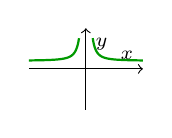
\begin{tikzpicture}
                            \begin{axis}[
                                    axis lines=middle,
                                    axis line style={->},
                                    xlabel={$x$},
                                    ylabel={$y$},
                                    label style={font=\scriptsize},
                                    xmin=-5, xmax=5,
                                    ymin=-5, ymax=5,
                                    xtick distance=1,
                                    ytick distance=1,
                                    enlargelimits=false,
                                    clip=false,
                                    width=0.25\textwidth,
                                    xtick=\empty,        % keine x-Ticks
                                    ytick=\empty,
                                ]
                                % Beispielfunktion (kubisch), so dass f(2) ≈ -6.33
                                \addplot[
                                    domain=-5:-0.6, samples=100, smooth,
                                    thick, green!60!black
                                ]
                                {1/x^2+1};
                                \addplot[
                                    domain=0.6:5, samples=100, smooth,
                                    thick, green!60!black
                                ]
                                {1/x^2+1};
                            \end{axis}
                        \end{tikzpicture}
                  \item 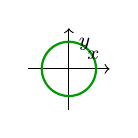
\begin{tikzpicture}
                            \begin{axis}[
                                    axis lines=middle,
                                    axis line style={->},
                                    xlabel={$x$},
                                    ylabel={$y$},
                                    label style={font=\scriptsize},
                                    xmin=-1.5, xmax=1.5,
                                    ymin=-1.5, ymax=1.5,
                                    xtick distance=1,
                                    ytick distance=1,
                                    enlargelimits=false,
                                    clip=false,
                                    width=0.25\textwidth,
                                    axis equal image,
                                    xtick=\empty,        % keine x-Ticks
                                    ytick=\empty,
                                ]
                                \addplot[
                                    domain=0:360, samples=100, smooth,
                                    thick, green!60!black
                                ]
                                ({cos(x)}, {sin(x)});
                            \end{axis}
                        \end{tikzpicture}
              \end{enumerate}
          \end{multicols}
    \item Ist die grafisch dargestellte Zuordnung $x \mapsto y$ eine Funktion?
          \begin{multicols}{3}
              \begin{enumerate}[label=\roman*)]
                  \item 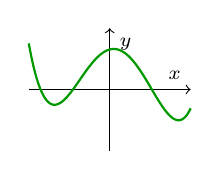
\begin{tikzpicture}
                            \begin{axis}[
                                    axis lines=middle,
                                    axis line style={->},
                                    xlabel={$x$},
                                    ylabel={$y$},
                                    label style={font=\scriptsize},
                                    xmin=-11, xmax=11,
                                    ymin=-20, ymax=20,
                                    xtick distance=1,
                                    ytick distance=20,
                                    enlargelimits=false,
                                    clip=false,
                                    width=0.3\textwidth,
                                    xtick=\empty,        % keine x-Ticks
                                    ytick=\empty,
                                ]

                                % Beispielfunktion (kubisch), so dass f(2) ≈ -6.33
                                \addplot[
                                    domain=-11:11, samples=100, smooth,
                                    thick, green!60!black
                                ]
                                {16/3/52.1*(-x+11.2)*(-x+7)*(1/5*(-x+7)-2.9)^2-5};
                            \end{axis}
                        \end{tikzpicture}
                  \item 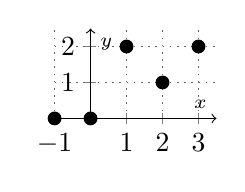
\begin{tikzpicture}
                            \begin{axis}[
                                    axis lines=middle,
                                    axis line style={->},
                                    xlabel={$x$},
                                    ylabel={$y$},
                                    label style={font=\scriptsize},
                                    xmin=-1, xmax=3.5,
                                    ymin=0, ymax=2.5,
                                    xtick distance=1,
                                    ytick distance=1,
                                    enlargelimits=false,
                                    clip=false,
                                    width=0.3\textwidth,
                                    grid=both,
                                    axis equal image,
                                    major grid style={line width=0.6pt,draw=black!60, dotted},
                                ]
                                % Beispielfunktion (kubisch), so dass f(2) ≈ -6.33
                                \fill (-1,0) circle (2.5pt);
                                \fill (0,0) circle (2.5pt);
                                \fill (1,2) circle (2.5pt);
                                \fill (2,1) circle (2.5pt);
                                \fill (3,2) circle (2.5pt);
                            \end{axis}
                        \end{tikzpicture}
                  \item 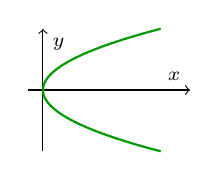
\begin{tikzpicture}
                            \begin{axis}[
                                    axis lines=middle,
                                    axis line style={->},
                                    xlabel={$x$},
                                    ylabel={$y$},
                                    label style={font=\scriptsize},
                                    xmin=-0.5, xmax=5,
                                    ymin=-2, ymax=2,
                                    xtick distance=1,
                                    ytick distance=1,
                                    enlargelimits=false,
                                    clip=false,
                                    width=0.3\textwidth,
                                    xtick=\empty,        % keine x-Ticks
                                    ytick=\empty,
                                ]
                                % Beispielfunktion (kubisch), so dass f(2) ≈ -6.33
                                \addplot[
                                    domain=-2:2, samples=100, smooth,
                                    thick, green!60!black
                                ]
                                ({x^2},{x});
                            \end{axis}
                        \end{tikzpicture}
              \end{enumerate}
          \end{multicols}

    \item Liegt der Punkt exakt auf dem Graphen von $f$ mit $f(x)=\sqrt{2-x}$?
          \begin{multicols}{3}
              \begin{enumerate}
                  \item $A=(0,1.4)$
                  \item $B=(-2,-2)$
                  \item $C=(-14,4)$
              \end{enumerate}
          \end{multicols}
    \item \begin{minipage}[t]{0.45\textwidth}
              Gegeben ist der Graph einer Funktion $f: x \mapsto y = f(x)$. Antworten Sie anhand der nebenstehenden Darstellung.
              \begin{enumerate}
                  \item Für welche Argumente $x$ ist $f(x)=3$?
                  \item Für welche Stellen $x$ ist $y=0$?
                  \item Welchen Wert hat $f(2)$ und welchen Wert hat $f(5)$?
              \end{enumerate}
          \end{minipage}
          \begin{minipage}[t]{0.5\textwidth}
              \vspace{0pt}
              \begin{center}
                  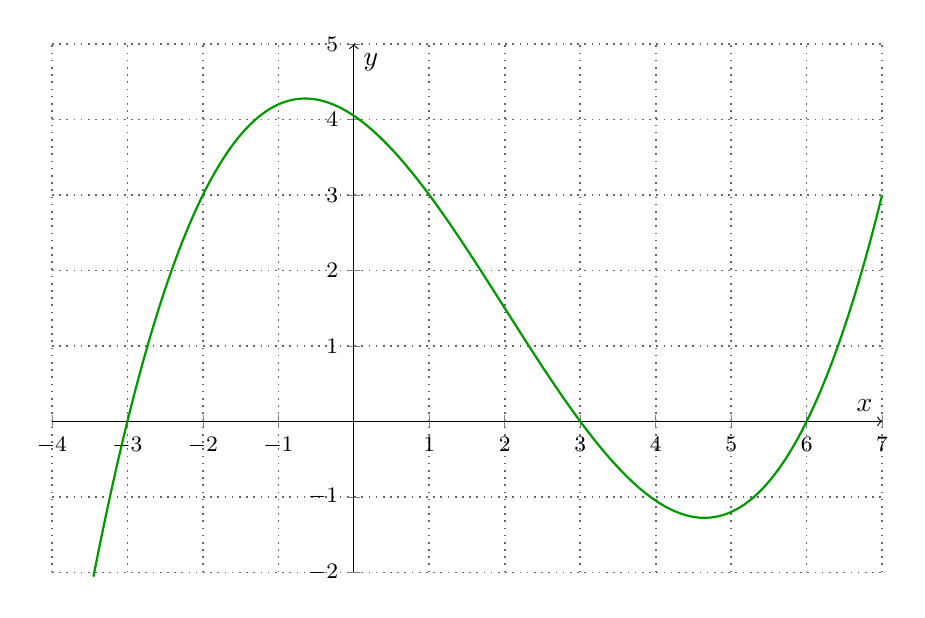
\begin{tikzpicture}
                      \begin{axis}[
                              axis lines=middle,
                              axis line style={->},
                              xlabel={$x$},
                              ylabel={$y$},
                              tick label style={font=\footnotesize},
                              xmin=-4, xmax=7,
                              ymin=-2, ymax=5,
                              xtick distance=1,
                              ytick distance=1,
                              enlargelimits=false,
                              clip=false,
                              width=\textwidth,
                              grid=both,
                              axis equal image,
                              major grid style={line width=0.6pt,draw=black!60, dotted},
                          ]
                          \addplot[
                              domain=-3.45:7, samples=100, smooth,
                              thick, green!60!black
                          ]
                          {((3)/(40))*(x+3)*(x-3)*(x-6)};
                      \end{axis}
                  \end{tikzpicture}
              \end{center}
          \end{minipage}
    \item Erstellen Sie eine Wertetabelle und zeichnen Sie den Graphen der folgenden Funktionen:
          \begin{multicols}{3}
              \begin{enumerate}
                  \item \( a(x) = \frac{x}{2} \)
                  \item \( b(x) = -\frac{1}{3}x + 6 \)
                  \item \( c(x) = 2\sqrt{x} \)
                        %   \item \( d(x) = -3\sqrt{x} \)
                  \item \( d(x) = \frac{5}{x + 3} \)
                  \item \( e(x) = \frac{1}{2}x^2 - \frac{9}{2} \)
                        %   \item \( g(x) = \sqrt{2x + 7} \)
              \end{enumerate}
          \end{multicols}
    \item Zeichnen Sie die Graphen der folgenden Funktionen \textbf{ohne Wertetabelle}. \\
          \textit{Tipp: Überlegen Sie, wie sich jeder Graph ab Aufgabe b) von dem davor unterscheidet.}
          \begin{enumerate}
              \item \( x \mapsto |x| \)
              \item \( x \mapsto -|x| \)
              \item \( x \mapsto -|x| + 1 \)
              \item \( x \mapsto |-\,|x| + 1| \)
          \end{enumerate}

    \item Welcher Graph gehört zu welcher Funktion?
          \begin{center}
              \pgfplotsset{
                  myaxis/.style={
                          axis lines=middle,
                          width=6cm, height=4.5cm,
                          samples=200,
                          xmin=-4.5, xmax=8.3,
                          ymin=-3, ymax=7,
                          xtick distance=2,
                          ytick distance=1,
                          enlargelimits=false,
                          tick label style={font=\scriptsize},
                      }
              }

              \begin{tikzpicture}
                  \begin{groupplot}[
                          myaxis,
                          group style={
                                  group size=3 by 3,
                                  horizontal sep=1.3cm,
                                  vertical sep=1.3cm
                              }
                      ]

                      % 1) y = x
                      \nextgroupplot[title={a)}, domain=-4:8,xtick distance=1, grid=both]
                      \addplot[draw=black, line width=0.3pt] {x};

                      % 2) y = sqrt(x-1)
                      \nextgroupplot[title={b)}, domain=1:9.5, xmin=-0.7, xmax=9.5, ymin =-0.5, ymax=5.8,xtick distance=1, grid=both]
                      \addplot[draw=black, line width=0.3pt] {sqrt(x-1)};

                      % 3) y = -1.2x + 3
                      \nextgroupplot[title={c)}, domain=-4:8, xtick distance=1, grid=both]
                      \addplot[draw=black, line width=0.3pt] {-1.2*x + 3};

                      % 4) y = 1.5^x
                      \nextgroupplot[title={d)}, domain=-4:8, xtick distance=1, grid=both]
                      \addplot[draw=black, line width=0.3pt] {1.5^x};

                      % 5) y = 0.5x^2 - 1.5x
                      \nextgroupplot[title={e)}, domain=-4:8, xtick distance=1, grid=both]
                      \addplot[draw=black, line width=0.3pt] {0.5*x^2 - 1.5*x};

                      % 6) y = 0.7x - 2
                      \nextgroupplot[title={f)}, domain=-4:8, xtick distance=1, grid=both]
                      \addplot[draw=black, line width=0.3pt] {0.7*x - 2};

                      % 7) y = 2/(x+1)
                      \nextgroupplot[title={g)}, domain=-4:8, xtick distance=1, grid=both]
                      \addplot[draw=black, line width=0.3pt, domain=-4:-1.01] {2/(x+1)};
                      \addplot[draw=black, line width=0.3pt, domain=-0.99:8] {2/(x+1)};
                  \end{groupplot}
              \end{tikzpicture}
          \end{center}

          \vspace{1em}
          \begin{multicols}{4}
              \begin{enumerate}[label=(\roman*)]
                  \item \( y = 0.7x - 2 \)
                  \item \( y = -1.2x + 3 \)
                  \item \( y = x \)
                  \item \( y = \dfrac{2}{x+1} \)
                  \item \( y = 0.5x^{2} - 1.5x \)
                  \item \( y = 1.5^{x} \)
                  \item \( y = \sqrt{x-1} \)
              \end{enumerate}
          \end{multicols}
    \item Zeichnen Sie den Graphen der folgenden Funktion:

          \( y = \operatorname{sgn}(x) \) (Vorzeichenfunktion; vgl. Aufgabe~\ref{aufgabe:vorzeichenfunktion} auf Seite ~\pageref{aufgabe:vorzeichenfunktion})

    \item \textbf{Challenge:} \( k:\; x \mapsto \sqrt{\,9 - (x-3)^2\,} \)
          \begin{enumerate}
              \item Bestimmen Sie den Definitionsbereich und die Wertemenge von \(k\).
              \item Erstellen Sie eine Wertetabelle für die zulässigen ganzzahligen Argumente.
              \item Skizzieren Sie den Graphen von \(k\).
              \item Um welche spezielle Kurve handelt es sich beim Graphen?
              \item Beweisen Sie die Vermutung aus d) wie folgt:
                    \begin{enumerate}
                        \item[i)] Betrachten Sie einen beliebigen Punkt \(P=(u, v)\) auf dem Graphen von \(k\).
                        \item[ii)] Berechnen Sie den Abstand zum Mittelpunkt mit Pythagoras.
                        \item[iii)] Formen Sie den Term aus ii) um, bis Sie das gewünschte Resultat erhalten.
                    \end{enumerate}
          \end{enumerate}
\end{enumerate}
\newpage
\subsection{Lösungen}
\begin{enumerate}
    \item i), iii)
    \item \begin{multicols}{3}\begin{enumerate}[label=\roman*)]
                  \item Funktion
                  \item Funktion
                  \item keine Funktion
              \end{enumerate}
          \end{multicols}
    \item \begin{multicols}{3}\begin{enumerate}
                  \item nein
                  \item nein
                  \item ja
              \end{enumerate}
          \end{multicols}
    \item \begin{multicols}{3}
              \begin{enumerate}
                  \item $x=-2$, $x=1$ und $x=7$
                  \item $x=-3$, $x=3$ und $x=6$
                  \item $f(2)\approx 1.5$, $f(5)\approx -1.2$
              \end{enumerate}
          \end{multicols}
    \item 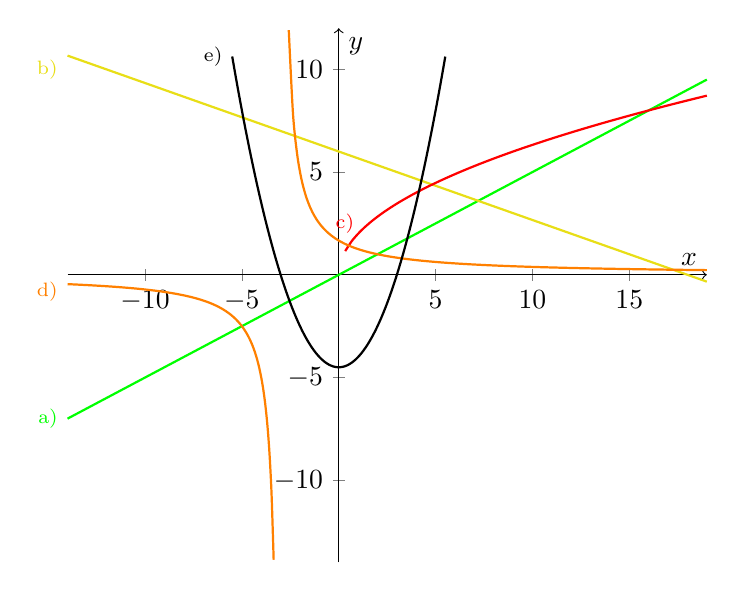
\begin{tikzpicture}[baseline=(current bounding box.north)]
              \begin{axis}[
                      axis lines=middle,
                      axis line style={->},
                      xlabel={$x$},
                      ylabel={$y$},
                      xmin=-14, xmax=19,
                      ymin=-14, ymax=12,
                      xtick distance=5,
                      ytick distance=5,
                      enlargelimits=false,
                      clip=false,
                      width=0.8\textwidth
                  ]

                  % Beispielfunktion (kubisch), so dass f(2) ≈ -6.33
                  \addplot[
                      domain=-14:19, samples=100, smooth,
                      thick, green
                  ]
                  {x/2};
                  \node[green, font=\scriptsize, left]
                  at (axis cs:-14,-7) {a)};
                  \addplot[
                      domain=-14:19, samples=100, smooth,
                      thick, yellow!90!black
                  ]
                  {-1/3*x+6};
                  \node[yellow!90!black, font=\scriptsize, left]
                  at (axis cs:-14,10) {b)};
                  \addplot[
                      domain=-14:19, samples=100, smooth,
                      thick, red
                  ]
                  {2*sqrt(x)};
                  \node[red, font=\scriptsize, left]
                  at (axis cs:1.3,2.5) {c)};
                  %   \addplot[
                  %       domain=-14:19, samples=100, smooth,
                  %       thick, blue
                  %   ]
                  %   {-3*sqrt(x)};
                  %   \node[blue, font=\scriptsize, right]
                  %   at (axis cs:19,-13) {d)};
                  \addplot[
                      domain=-14:-3.36, samples=100, smooth,
                      thick, orange
                  ]
                  {5/(x+3)};
                  \addplot[
                      domain=-2.58:19, samples=100, smooth,
                      thick, orange
                  ]
                  {5/(x+3)};
                  \node[orange, font=\scriptsize, left]
                  at (axis cs:-14,-0.8) {d)};
                  \addplot[
                      domain=-5.5:5.5, samples=100, smooth,
                      thick, black
                  ]
                  {1/2*x*x-9/2};
                  \node[black, font=\scriptsize, left]
                  at (axis cs:-5.5,10.625) {e)};
                  %   \addplot[
                  %       domain=-3.5:19, samples=100, smooth,
                  %       thick, black
                  %   ]
                  %   {sqrt(2*x+7)};
                  %   \node[black, font=\scriptsize, right]
                  %   at (axis cs:19,6.5) {f)};
              \end{axis}
          \end{tikzpicture}
    \item \pgfplotsset{
              myaxis/.style={
                      axis lines=middle,
                      width=6cm, height=6cm,
                      samples=100,
                      xmin=-5.5, xmax=5.5,
                      ymin=-5.5, ymax=5.5,
                      xtick distance=1,
                      ytick distance=1,
                      grid=major,
                      enlargelimits=false,
                      tick label style={font=\scriptsize},
                  }
          }

          \begin{tikzpicture}[baseline=(current bounding box.north)]
              \begin{groupplot}[
                      myaxis,
                      group style={
                              group size=2 by 2,
                              horizontal sep=1.3cm,
                              vertical sep=1.3cm
                          }
                  ]

                  \nextgroupplot[title={a)}]
                  \addplot[draw=black, line width=0.3pt] {abs(x)};

                  \nextgroupplot[title={b)}]
                  \addplot[draw=black, line width=0.3pt] {-abs(x)};

                  \nextgroupplot[title={c)}]
                  \addplot[draw=black, line width=0.3pt] {-abs(x)+1};

                  \nextgroupplot[title={d)}]
                  \addplot[draw=black, line width=0.3pt] {abs(-abs(x)+1)};
              \end{groupplot}
          \end{tikzpicture}
    \item a) $\leftrightarrow$ iii);  b) $\leftrightarrow$ vii);  c) $\leftrightarrow$ ii);  d) $\leftrightarrow$ vi);  e) $\leftrightarrow$ v);  f) $\leftrightarrow$ i);  g) $\leftrightarrow$ iv)
    \item \begin{tikzpicture}[baseline=(current bounding box.north)]
              \begin{groupplot}[
                      axis lines=middle,
                      width=6cm, height=4cm,
                      samples=100,
                      ymin=-3, ymax=3,
                      xtick distance=1,
                      ytick distance=1,
                      grid=major,
                      enlargelimits=false,
                      tick label style={font=\scriptsize},
                      group style={
                              group size=2 by 1,
                              horizontal sep=1.3cm,
                              vertical sep=1.3cm
                          }
                  ]

                  \nextgroupplot[title={$y=\operatorname{sgn}(x)$}]
                  \addplot[domain=-5.5:-0.1, draw=red, line width=0.3pt] {sign(x)};
                  \addplot[domain=0.1:5.5, draw=red, line width=0.3pt] {sign(x)};
                  \fill[red] (axis cs:0,0) circle (1.5pt);
              \end{groupplot}
          \end{tikzpicture}
    \item Challenge:
          \begin{enumerate}
              \item[a)] \(\mathbb{D}=[0,6],\qquad \mathbb{W}=[0,3]\)

              \item[b)] \textbf{Wertetabelle}\\[2mm]
                    \renewcommand{\arraystretch}{1.3}
                    \setlength{\tabcolsep}{10pt}
                    \begin{tabular}{|c|c|c|c|c|c|c|c|}
                        \hline
                        \(x\)    & 0                         & 1                         & 2                         & 3 & 4 & 5 & 6 \\
                        \hline
                        \(k(x)\) & 0                         & \(\sqrt{5}\approx 2{,}2\) & \(\sqrt{8}\approx 2{,}8\) & 3
                                 & \(\sqrt{8}\approx 2{,}8\) & \(\sqrt{5}\approx 2{,}2\) & 0                                         \\
                        \hline
                    \end{tabular}

              \item[c)] \textbf{Graph:}\\[2mm]
                    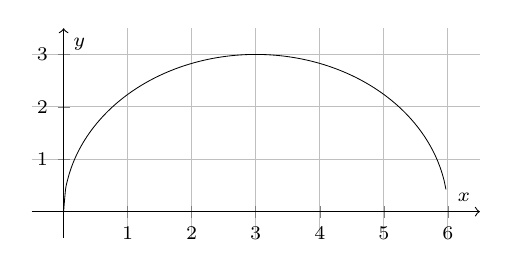
\begin{tikzpicture}
                        \begin{axis}[
                                axis lines=middle,
                                axis line style={->},
                                xmin=-0.5, xmax=6.5,
                                ymin=-0.5, ymax=3.5,
                                xtick={0,1,2,3,4,5,6},
                                ytick={0,1,2,3},
                                grid=both,
                                width=0.6\textwidth,
                                height=0.35\textwidth,
                                tick label style={font=\scriptsize},
                                label style={font=\scriptsize},
                                xlabel={$x$}, ylabel={$y$}
                            ]
                            \addplot[domain=0:6, samples=200, smooth, draw=black, line width=0.3pt]
                            {sqrt(9 - (x-3)^2)};
                        \end{axis}
                    \end{tikzpicture}

              \item[d)] Es ist ein \textbf{Halbkreis} (oberer Halbkreis mit Mittelpunkt \(M=(3,0)\) und Radius \(r=3\)).

              \item[e)]             Sei \(P=(u, v)\) ein beliebiger Punkt auf dem Graphen von \(k\).\\
                    Abstand von \(P\) zum Mittelpunkt \(M=(3, 0)\):
                    \[
                        d=\sqrt{(u-3)^2+v^2}.
                    \]
                    Da \(P\) auf dem Graphen von \(k\) liegt, gilt \(v=\sqrt{\,9-(3-u)^2\,}\). Also
                    \[
                        d=\sqrt{(u-3)^2+\left(\sqrt{\,9-(3-u)^2\,}\right)^2}
                        =\sqrt{(u-3)^2+9-(3-u)^2}.
                    \]
                    Da $(u-3)=-(3-u)$ ist, gilt \((u-3)^2=(3-u)^2\), somit streichen sich die beiden Klammern unter der Wurzel weg:
                    \[
                        d=\sqrt{9}=3.
                    \]
                    Damit haben alle Punkte des Graphen von \(k\) den Abstand \(3\) zu \(M\).
          \end{enumerate}
\end{enumerate}
\newpage

\section{Eigenschaften von Funktionsgraphen}
\subsection{Achsenschnittpunkte}
\subsubsection{Einstiegsaufgabe}
Funktionsgraphen sind unter anderem deshalb so nützlich, weil einige Besonderheiten und Eigenschaften der Funktion auf einen Blick sichtbar werden.

Um zwei wichtige Merkmale einer Funktion geht's nun im Folgenden: y-Achsenabschnitt und Nullstellen.
\bigskip

Gegeben sei folgende Funktion:
\[f(x) = -2x^2 + 8x + 10\]

\begin{enumerate}
    \item Vervollständigen Sie die Wertetabelle:
          \begin{center}
              \renewcommand{\arraystretch}{1.8} % Erhöht die Zeilenhöhe um den Faktor 1.8
              \begin{tabular}{|p{1cm}|p{1cm}|p{1cm}|p{1cm}|p{1cm}|p{1cm}|p{1cm}|p{1cm}|p{1cm}|p{1cm}|}
                  \hline
                  $x$    & $-2$  & $-1$ & $0$ & $1$ & $2$ & $3$ & $4$ & $5$ & $6$   \\
                  \hline
                  $f(x)$ & $-14$ &      &     &     &     &     &     &     & $-14$ \\
                  \hline
              \end{tabular}
          \end{center}
    \item Zeichnen Sie den Graphen der Funktion
          \begin{center}
              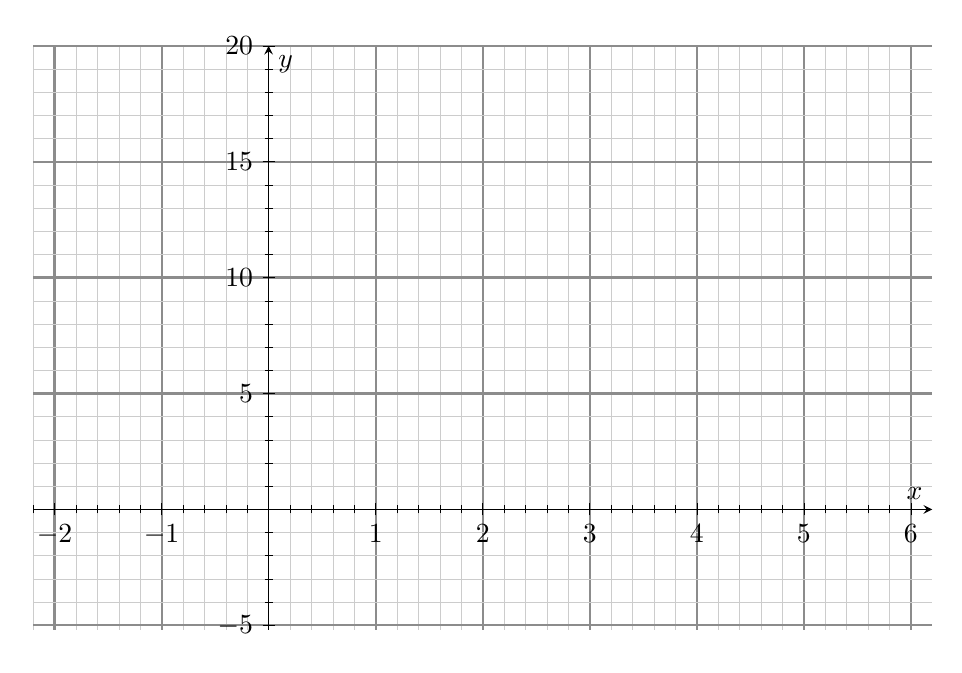
\begin{tikzpicture}
                  \begin{axis}[
                          width=13cm, height=9cm,
                          axis lines=middle,
                          axis line style={-stealth},
                          xlabel={$x$}, ylabel={$y$},
                          xmin=-2.2, xmax=6.2,
                          ymin=-5.2,  ymax=20,
                          xtick={-3,-2,-1,0,1,2,3,4,5,6},
                          ytick={-5,0,5,10,15,20,25,30,35},
                          %xticklabels={$-3$,$-2$,$-1$,$0$,$1$,$2$,$3$,$4$,$5$},
                          %yticklabels={$-5$,$0$,},
                          grid=both,
                          minor tick num=4,
                          tick style={black},
                          enlargelimits=false,
                          major grid style={line width=0.8pt, draw=gray!90},
                          minor grid style={line width=0.2pt, draw=gray!40},
                      ]
                      % kein Funktionsgraph – nur das Koordinatensystem
                  \end{axis}
              \end{tikzpicture}
          \end{center}
    \item Die $y$-Koordinate des Schnittpunktes eines Funktionsgraphen mit der y-Achse heisst \textbf{y-Achsenabschnitt}. Lesen Sie den y-Achsenabschnitt von $f$ am Graphen ab.
    \item Wie hätte man den y-Achsenabschnitt von $f$ berechnen können?
    \item Die x-Koordinaten der Schnittpunkte eines Funktionsgraphen mit der x-Achse heissen \textbf{Nullstellen}. Lesen Sie die Nullstellen von $f$ am Graphen ab.
    \item Challenge: Welche Gleichung müsste man lösen, um die Nullstellen von $f$ zu berechnen?
\end{enumerate}
\newpage

\begin{deff}[Nullstelle]{}
    Sei \( f : \D \to \W \) eine Funktion.
    Ein Input \( x_0 \in \D \) mit der Eigenschaft, dass
    \[
        f(x_0) = 0
    \]
    ist, heisst \textbf{Nullstelle} der Funktion.

    \medskip

    Die Nullstellen sind diejenigen Stellen, an denen der Graph der Funktion die \(x\)-Achse schneidet.
\end{deff}
\begin{example}
    Bestimmen Sie die Nullstellen der Funktion
    \[f(x) = -2x^2 + 8x + 10\]
    \kariert{10}
    \begin{center}
        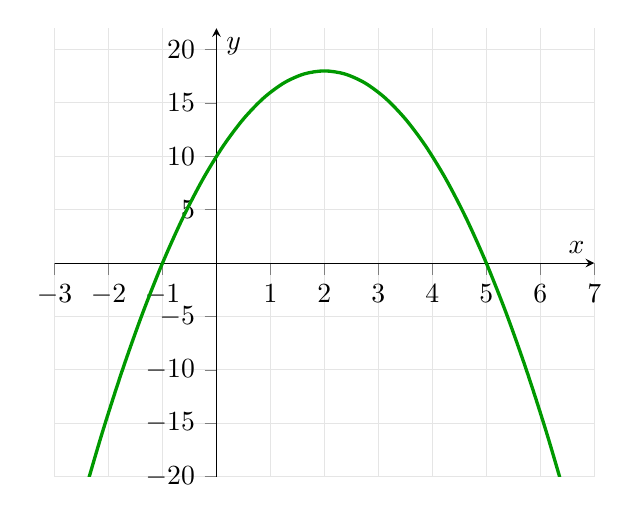
\begin{tikzpicture}
            \begin{axis}[
                    axis lines=middle,
                    xlabel={$x$},
                    ylabel={$y$},
                    xmin=-3, xmax=7,
                    ymin=-20, ymax=22,
                    xtick={-3,-2,-1,0,1,2,3,4,5,6,7},
                    ytick={-20,-15,-10,-5,0,5,10,15,20},
                    grid=both,
                    %minor tick num=4,
                    grid style={lightgray!40},
                    tick align=outside,
                    enlargelimits=false,
                ]
                % Parabel (anpassen, falls du eine andere Form willst)
                \addplot[
                    domain=-2.5:6.5,
                    very thick,
                    smooth,
                    color=green!60!black
                ] {-2*(x)^2 + 8*x + 10};
            \end{axis}
        \end{tikzpicture}
    \end{center}
\end{example}
Auch der Schnittpunkt mit der vertikalen Achse hat einen eigenen Namen:
\begin{deff}[y-Achsenabschnitt]{}
    Sei \( f : D \to W \) eine Funktion.
    Die \( y \)-Koordinate \( y_0 \in W \) des Schnittpunktes des Graphen mit der \( y \)-Achse
    heisst \textbf{\( y \)-Achsenabschnitt}.

    \medskip

    Der \( y \)-Achsenabschnitt ist der Funktionswert an der Stelle $x=0$:
    \[
        y_0 = f(0)
    \]
\end{deff}

Die Funktion $f$ aus dem Beispiel oben hat den y-Achsenabschnitt $y_0=f(0)=10$.

\begin{example}
    \begin{minipage}{0.6\textwidth}
        Nicht jede Funktion hat Nullstellen und/oder einen y-Achsenabschnitt:
        \[g(x)=\sqrt{x-1}+2\]
        Hat weder das eine noch das andere (siehe Bild).
    \end{minipage}
    \begin{minipage}{0.4\textwidth}
        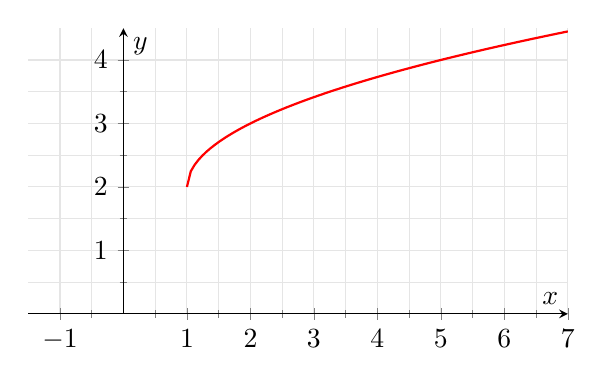
\begin{tikzpicture}
            \begin{axis}[
                    axis lines=middle,
                    xlabel={$x$},
                    ylabel={$y$},
                    xmin=-1.5, xmax=7,
                    ymin=0, ymax=4.5,
                    xtick={-1,0,1,2,3,4,5,6,7},
                    ytick={0,1,2,3,4},
                    grid=both,
                    minor tick num=1,
                    grid style={lightgray!40},
                    samples=100,
                    domain=1:7,
                    axis equal image
                ]
                % Funktionsgraph
                \addplot[
                    thick,
                    red
                ] {sqrt(x - 1) + 2};
            \end{axis}
        \end{tikzpicture}
    \end{minipage}
\end{example}


\newpage
\subsection{Übungen}
\begin{enumerate}
    \item Berechnen Sie jeweils die Nullstelle(n) und den y-Achsenabschnitt.
          \begin{enumerate}
              \item \( f(x) = \tfrac{3}{10}x - 6 \)
              \item \( g(x) = -x^2 + 9 \)
              \item \( h(x) = x^3 - x \)
              \item \(i(x)=3\)
              \item \(y=|x|\)
              \item \( y = \operatorname{sgn}(x) \) (Vorzeichenfunktion; vgl. Aufgabe~\ref{aufgabe:vorzeichenfunktion} auf Seite ~\pageref{aufgabe:vorzeichenfunktion})
          \end{enumerate}
    \item \begin{enumerate}
              \item Erklären Sie, weshalb eine Funktion maximal einen y-Achsenabschnitt haben kann.
              \item Unter welcher Bedingung hat eine Funktion keinen y-Achsenabschnitt?
          \end{enumerate}
    \item Geben Sie eine möglichst einfache Funktion an mit
          \begin{enumerate}
              \item y-Achsenabschnitt \( y_0 = 5 \).
              \item y-Achsenabschnitt \( y_0 = 2 \) und Nullstelle \( x_0 = 4 \).
              \item den Nullstellen \( x_1 = -2,\, x_2 = 2 \).
              \item ohne Nullstellen.
              \item ohne y-Achsenabschnitt.
          \end{enumerate}
\end{enumerate}
\newpage
\subsection{Lösungen}
\begin{enumerate}
    \item \begin{enumerate}
              \item Nullstelle: \(x = 20\), y-Achsenabschnitt: \(y_0 = -6\)
              \item Nullstelle: \(x_1 = -3, x_2 = 3\); y-Achsenabschnitt: \(y_0 = 9\)
              \item Nullstelle: \(x_1 = -1, x_2 = 0, x_3 = 1\); y-Achsenabschnitt: \(y_0 = 0\)
              \item Nullstelle: keine; y-Achsenabschnitt: \(y_0 = 3\)
              \item Nullstelle: \(x=0\); y-Achsenabschnitt: \(y_0 = 0\)
              \item Nullstelle: \(x=0\); y-Achsenabschnitt: \(y_0 = 0\)
          \end{enumerate}
    \item \begin{enumerate}
              \item Zwei y-Achsenabschnitte würde bedeuten, dass die Funktion an der Stelle $x=0$ zwei Funktionswerte hat.
              \item Wenn $0 \notin \D$.
          \end{enumerate}
    \item Mögliche Antworten:
          \begin{enumerate}
              \item \(y = 5\)
              \item \(y = -\tfrac{1}{2}x + 2\)
              \item \(y = x^2 - 4\)
              \item \(y = 5\)
              \item \(y = \tfrac{1}{x}\) ($0 \notin \D$)
          \end{enumerate}
\end{enumerate}
\newpage
\subsection{Monotonie}
Oft ist es wichtig zu wissen, ob die Funktionswerte in einem bestimmten Teilbereich der Definitionsmenge ansteigen oder fallen.
\begin{deff}[Monotonie]{}
    Eine Funktion \( f : \D \to \W \) heisst \textbf{monoton wachsend}, falls für alle \( x_1 < x_2 \in \D \) folgt, dass
    \[
        f(x_1) \le f(x_2)
    \]
    ist.

    Sie heisst \textbf{streng monoton wachsend}, falls für alle \( x_1 < x_2 \in \D \) folgt, dass
    \[
        f(x_1) < f(x_2)
    \]
    ist.

    \medskip

    Analog werden auch die Begriffe \textbf{monoton fallend} und \textbf{streng monoton fallend} definiert.
\end{deff}

\begin{example}
    Die Funktion $y=-x^3$ ist streng monoton fallend:
    \begin{center}
        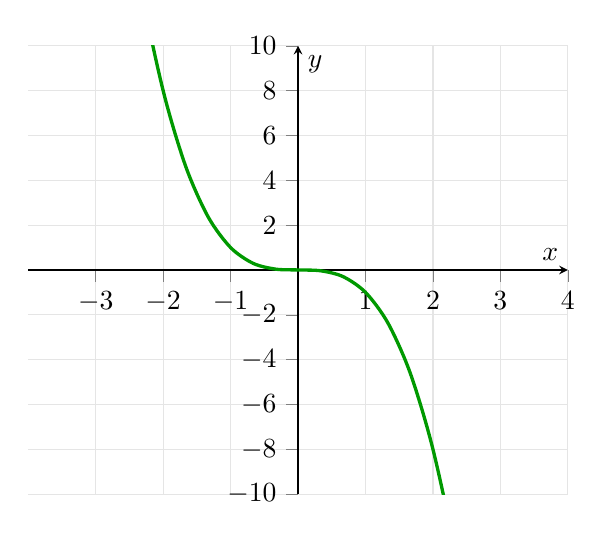
\begin{tikzpicture}
            \begin{axis}[
                    axis lines=middle,
                    xlabel={$x$},
                    ylabel={$y$},
                    xmin=-4, xmax=4,
                    ymin=-10, ymax=10,
                    xtick={-3,-2,-1,0,1,2,3,4,5,6,7},
                    ytick={-10,-8,...,10},
                    grid=both,
                    %minor tick num=4,
                    grid style={lightgray!40},
                    tick align=outside,
                    enlargelimits=false,
                ]
                % Parabel (anpassen, falls du eine andere Form willst)
                \addplot[
                    domain=-4:4,
                    very thick,
                    smooth,
                    color=green!60!black
                ] {-x^3};
            \end{axis}
        \end{tikzpicture}
    \end{center}
\end{example}

\begin{example}
    Die Funktion aus der Einstiegsaufgabe des vorherigen Abschnittes ist streng monoton wachsend im Intervall $]-\infty,2]$ und streng monoton fallend im Bereich $[2,\infty[$.
    \begin{center}
        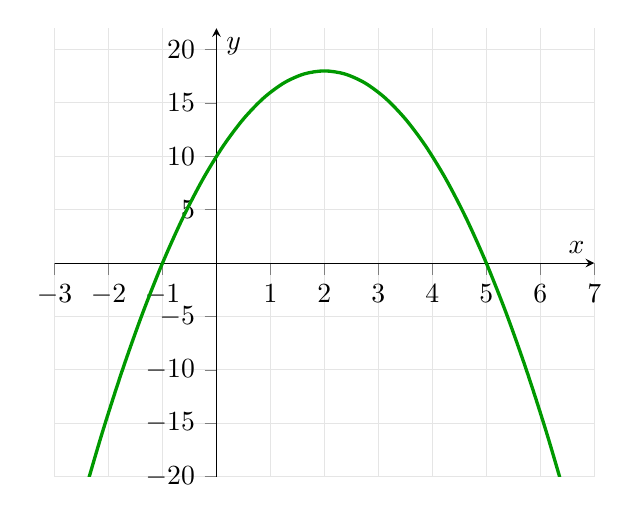
\begin{tikzpicture}
            \begin{axis}[
                    axis lines=middle,
                    xlabel={$x$},
                    ylabel={$y$},
                    xmin=-3, xmax=7,
                    ymin=-20, ymax=22,
                    xtick={-3,-2,-1,0,1,2,3,4,5,6,7},
                    ytick={-20,-15,-10,-5,0,5,10,15,20},
                    grid=both,
                    %minor tick num=4,
                    grid style={lightgray!40},
                    tick align=outside,
                    enlargelimits=false,
                ]
                % Parabel (anpassen, falls du eine andere Form willst)
                \addplot[
                    domain=-2.5:6.5,
                    very thick,
                    smooth,
                    color=green!60!black
                ] {-2*(x)^2 + 8*x + 10};
            \end{axis}
        \end{tikzpicture}
    \end{center}
\end{example}

\begin{example}
    Die Abrundungsfunktion wird mit \(\mathrm{floor}(x)\) oder \(\lfloor x\rfloor\) bezeichnet.
    Sie ordnet jeder reellen Zahl \(x\) die grösste ganze Zahl \(n\le x\) zu.
    Zum Beispiel \(\lfloor \pi\rfloor=3\) oder \(\left\lfloor -\tfrac34\right\rfloor=-1\) oder \(\lfloor 5\rfloor=5\).
    Der Graph der Abrundungsfunktion sieht wie folgt aus:

    \medskip

    \begin{center}
        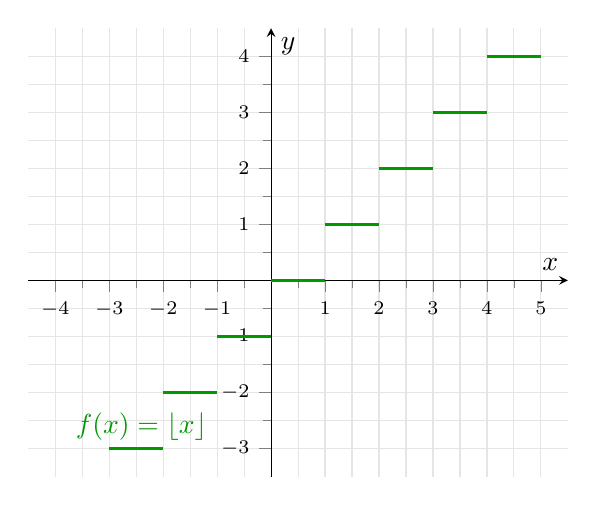
\begin{tikzpicture}
            \begin{axis}[
                    axis lines=middle,
                    xlabel={$x$}, ylabel={$y$},
                    xmin=-4.5, xmax=5.5,
                    ymin=-3.5, ymax=4.5,
                    xtick={-4,-3,-2,-1,0,1,2,3,4,5},
                    ytick={-3,-2,-1,0,1,2,3,4},
                    grid=both,
                    minor tick num=1,
                    grid style={lightgray!40},
                    tick align=outside,
                    tick label style={font=\scriptsize}
                ]

                % Stufen: für n = -3,...,4 wird [n,n+1) -> n gezeichnet
                \foreach \n in {-3,-2,-1,0,1,2,3,4}{
                        % horizontale Stufe
                        \addplot[
                            very thick,
                            green!60!black
                        ] coordinates {(\n,\n) (\n+1,\n)};
                    }

                % Beschriftung im Graphen
                \node[anchor=west, text=green!60!black] at (axis cs:-3.8,-2.6)
                {$f(x)=\lfloor x\rfloor$};

            \end{axis}
        \end{tikzpicture}
    \end{center}
    \medskip
    \noindent
    Die Abrundungsfunktion ist \textbf{monoton wachsend}, aber \textbf{nicht streng monoton wachsend}.
\end{example}
\newpage
\subsection*{Gerade und ungerade Funktionen}
\subsubsection{Einstiegsaufgabe}
Ziel der Aufgabe ist die Untersuchung von Funktionen mit Graphen, die punktsymmetrisch zum Ursprung oder achsensymmetrisch zur y-Achse verlaufen.
\begin{enumerate}
    \item Betrachten Sie den Punkt $P=(1,-3)$ im Koordinatensystem:
          \begin{center}
              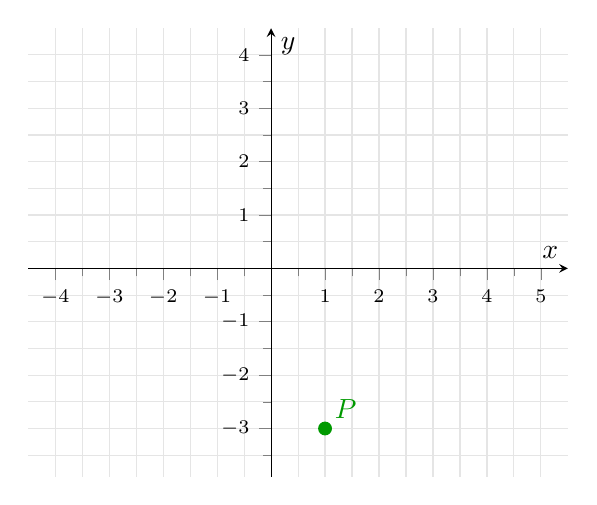
\begin{tikzpicture}
                  \begin{axis}[
                          axis lines=middle,
                          xlabel={$x$}, ylabel={$y$},
                          xmin=-4.5, xmax=5.5,
                          ymin=-3.9, ymax=4.5,
                          xtick={-4,-3,-2,-1,0,1,2,3,4,5},
                          ytick={-4,-3,-2,-1,0,1,2,3,4},
                          grid=both,
                          minor tick num=1,
                          grid style={lightgray!40},
                          tick align=outside,
                          tick label style={font=\scriptsize}
                      ]
                      % Beschriftung im Graphen
                      \node[anchor=south west, text=green!60!black] at (1,-3)
                      {$P$};
                      \fill[color=green!60!black] (1,-3) circle (2.5pt);
                  \end{axis}
              \end{tikzpicture}
          \end{center}
          Wohin kommt der Punkt $P$ zu liegen nach einer Punktspiegelung mit Zentrum im Ursprung $O=(0,0)$? Geben Sie die Koordinaten des Bildpunktes $P'$ an:
          \vspace{1cm}

    \item Gegeben ist nun die Funktion $f(x)=x(x-2)(x+2)$.
          \begin{enumerate}
              \item Weisen Sie rechnerisch nach, dass der Punkt $P$ aus Aufgabe 1. auf dem Graphen von $f$ liegt.
              \item Liegt auch der Punkt P' auf dem Graphen von f?
              \item Prüfen Sie nun, ob der Graphenpunkt $Q(3,?)$ und sein Spiegelpunkt $Q'$ beide auf dem Graphen von f liegen.
              \item Wieso reichen die Erkenntnisse aus den Teilaufgaben a)-c) nicht als Beweis, dass der Graph von f punktsymmetrisch zum Ursprung verläuft?
              \item Was müsste man prüfen, um Gewissheit über die Punktsymmetrie des Graphen zu erlangen?
          \end{enumerate}
    \item Betrachten Sie zum Schluss die Funktion $g(x)=\dfrac{1}{x^2+1}$. Alice behauptet, der Graph der Funktion $g$ verlaufe achsensymmetrisch bezüglich y-Achse. Stimmt ihre Behauptung?
\end{enumerate}
\newpage
\begin{example}
    Nachweis der Punktsymmetrie von $f(x)=x(x-2)(x+2)$:
    \smallskip

    \begin{minipage}{0.6\textwidth}
        \kariert{20}
    \end{minipage}
    \begin{minipage}{0.4\textwidth}
        \begin{center}
            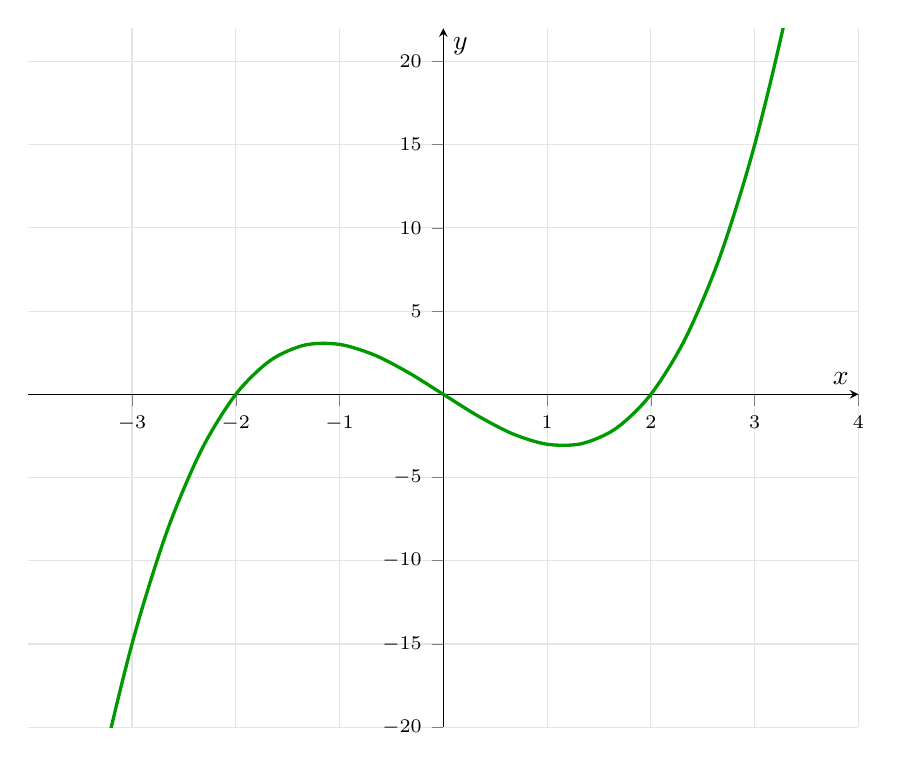
\begin{tikzpicture}
                \begin{axis}[
                        axis lines=middle,
                        xlabel={$x$},
                        ylabel={$y$},
                        xmin=-4, xmax=4,
                        ymin=-20, ymax=22,
                        xtick={-3,-2,-1,0,1,2,3,4,5,6,7},
                        ytick={-20,-15,-10,-5,0,5,10,15,20},
                        grid=both,
                        %minor tick num=4,
                        grid style={lightgray!40},
                        tick align=outside,
                        enlargelimits=false,
                        width=\textwidth,
                        tick label style={font=\scriptsize}
                    ]
                    % Parabel (anpassen, falls du eine andere Form willst)
                    \addplot[
                        domain=-4:4,
                        very thick,
                        smooth,
                        color=green!60!black
                    ] {x*(x-2)*(x+2)};
                \end{axis}
            \end{tikzpicture}
        \end{center}
    \end{minipage}
\end{example}
\smallskip

\begin{deff}[Ungerade Funktion]{}
    Falls für eine Funktion $f: \D\to \W$ gilt, dass
    \[f(-\varepsilon)=-f(\varepsilon) \text{ für alle } \varepsilon \in \D\]
    so verläuft der Graph der Funktion punktsymmetrisch zum Ursprung.

    Eine Funktion mit dieser Eigenschaft nennt man \textbf{ungerade}.
\end{deff}
Analog gibt es Funktionen deren Graphen achsensymmetrisch zur y-Achse verlaufen:
\begin{deff}[Gerade Funktion]{}
    Falls für eine Funktion $f: \D\to \W$ gilt, dass
    \[f(-\varepsilon)=f(\varepsilon) \text{ für alle } \varepsilon \in \D\]
    so verläuft der Graph der Funktion achsensymmetrisch zur y-Achse.

    Eine Funktion mit dieser Eigenschaft nennt man \textbf{gerade}.
\end{deff}
\begin{example}
    \begin{minipage}{0.6\textwidth}
        Die Funktion $g(x)=\dfrac{1}{x^2+1}$ ist gerade, denn
        \[
            g(\varepsilon)= \dfrac{1}{\varepsilon^2+1}, \quad g(-\varepsilon) = \dfrac{1}{(-\varepsilon)^2+1} = \dfrac{1}{\varepsilon^2+1}
        \]
        Also gilt für alle $\varepsilon \in \D$: $g(-\varepsilon) = g(\varepsilon)$.
    \end{minipage}
    \begin{minipage}{0.4\textwidth}
        \begin{center}
            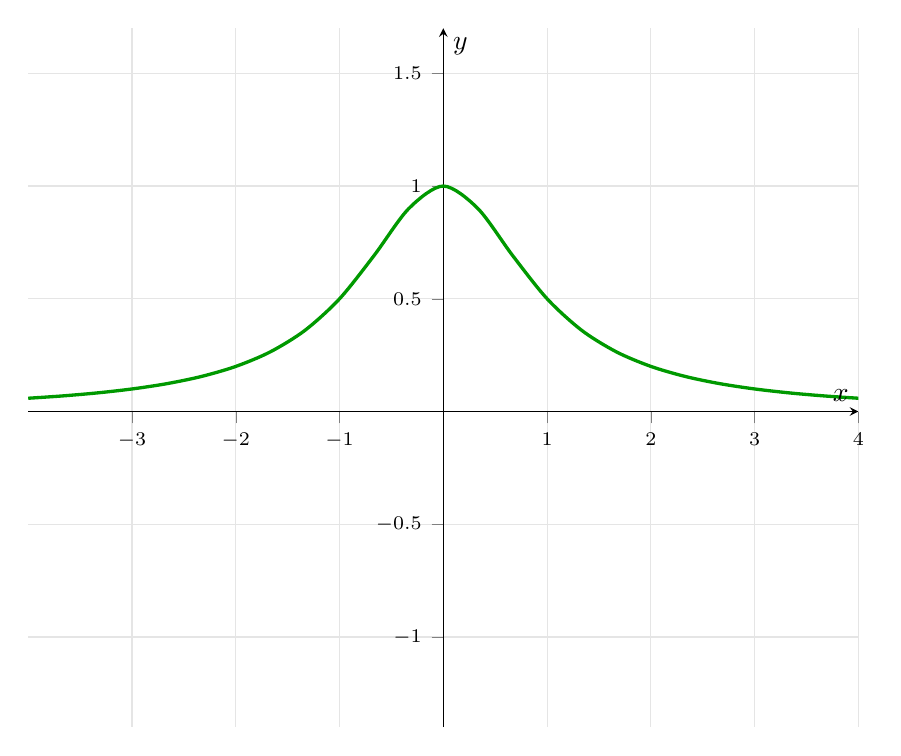
\begin{tikzpicture}
                \begin{axis}[
                        axis lines=middle,
                        xlabel={$x$},
                        ylabel={$y$},
                        xmin=-4, xmax=4,
                        ymin=-1.4, ymax=1.7,
                        xtick={-3,-2,-1,0,1,2,3,4,5,6,7},
                        ytick={-1,-0.5,0,0.5,1,1.5},
                        grid=both,
                        %minor tick num=4,
                        grid style={lightgray!40},
                        tick align=outside,
                        enlargelimits=false,
                        width=\textwidth,
                        tick label style={font=\scriptsize}
                    ]
                    % Parabel (anpassen, falls du eine andere Form willst)
                    \addplot[
                        domain=-4:4,
                        very thick,
                        smooth,
                        color=green!60!black
                    ] {1/(x^2+1)};
                \end{axis}
            \end{tikzpicture}
        \end{center}
    \end{minipage}
\end{example}
\vspace{1cm}

Neben den in diesem Kapitel besprochenen Eigenschaften von Graphen gibt es viele andere, die zum Teil zu einem späteren Zeitpunkt behandelt werden: Periodizität, Krümmungsverhalten, Wendepunkte, lokale Extrema, asymptotisches Verhalten und viele mehr...
\newpage

\subsubsection{Übungen}
\begin{enumerate}
    \item Entscheiden Sie, ob die Funktion insgesamt (streng) monoton wachsend oder fallend ist. Falls sie das nicht ist, identifizieren Sie bitte Intervalle, über denen sie (streng) monoton wachsend oder fallend ist.
          \begin{enumerate}
              \item $y=|x|$
              \item $y=\operatorname{sgn}(x)$
              \item $y=\sqrt{5x+16}$
              \item $y=x^2-4$
          \end{enumerate}
    \item Beweisen Sie die Aussagen:
          \begin{enumerate}
              \item $y=x$ ist ungerade.
              \item $y=-x^2+9$ ist gerade.
              \item $y=x^3-x$ ist ungerade
          \end{enumerate}
    \item Geben sie für jede der folgenden Funktionen Folgendes an:
          \begin{enumerate}[label=\roman*)]
              \item Definitionsbereich
              \item y-Achsenabschnitt
              \item alle Nullstellen
              \item gerade oder ungerade
              \item Teilmengen des Definitionsbereichs, auf welchen die
                    Funktion (streng) monoton wachsend oder fallend ist
          \end{enumerate}
          \begin{multicols}{2}
              \begin{enumerate}
                  \item $y=(x-2)^2$
                  \item $y=x^3$
                  \item $y=\dfrac{1}{x}$
                  \item $y=\sqrt{5x+16}$
              \end{enumerate}
          \end{multicols}
\end{enumerate}
\newpage
\subsubsection{Lösungen}
\begin{enumerate}
    \item Entscheiden Sie, ob die Funktion insgesamt (streng) monoton wachsend oder fallend ist. Falls sie das nicht ist, identifizieren Sie bitte Intervalle, über denen sie (streng) monoton wachsend oder fallend ist.
          \begin{enumerate}
              \item streng monoton fallend auf $]-\infty, 0]$, streng monoton wachsend auf $[0,\infty[$
              \item monoton wachsend, nicht aber streng monoton wachsend
              \item streng monoton wachsend
              \item streng monoton fallend auf $]-\infty, 2]$, streng monoton wachsend auf $[-2,\infty[$
          \end{enumerate}
    \item Beweisen Sie die Aussagen:
          \begin{enumerate}
              \item $f(-\varepsilon)=-\varepsilon$\\
                    $-f(\varepsilon) = -(\varepsilon) = -\varepsilon$ $\checkmark$
              \item $f(-\varepsilon)=-(-\varepsilon)^2+9 = -\varepsilon^2 + 9 = f(\varepsilon)$ \checkmark
              \item $f(-\varepsilon)=(-\varepsilon)^3-(-\varepsilon) = -\varepsilon^3 + \varepsilon$\\
                    $-f(\varepsilon) = -(\varepsilon^3 -\varepsilon) = -\varepsilon^3 + \varepsilon$ \checkmark
          \end{enumerate}
    \item Geben sie für jede der folgenden Funktionen Folgendes an:
          \begin{enumerate}[label=\roman*)]
              \item Definitionsbereich
              \item y-Achsenabschnitt
              \item alle Nullstellen
              \item gerade oder ungerade
              \item Teilmengen des Definitionsbereichs, auf welchen die
                    Funktion (streng) monoton wachsend oder fallend ist
          \end{enumerate}
          \begin{multicols}{2}
              \begin{enumerate}
                  \item \begin{enumerate}[label=\roman*)]
                            \item $\D=\R$
                            \item $y=4$
                            \item $x = 2$
                            \item weder gerade noch ungerade
                            \item monoton fallend: $]-\infty, 2]$, monoton wachsend: $[2, \infty[$
                        \end{enumerate}
                  \item \begin{enumerate}[label=\roman*)]
                            \item $\D=\R$
                            \item $y=0$
                            \item $x = 0$
                            \item ungerade
                            \item streng monoton wachsend
                        \end{enumerate}\columnbreak
                  \item \begin{enumerate}[label=\roman*)]
                            \item $\D=\R \setminus \{0\}$
                            \item existiert nicht, da $0\notin \D$
                            \item keine Nullstellen
                            \item ungerade
                            \item streng monoton fallend: $]0, \infty[$, streng monoton fallend: $]-\infty, 0[$\\
                                  Funktion als Ganzes aber nicht monoton fallend
                        \end{enumerate}
                  \item \begin{enumerate}[label=\roman*)]
                            \item $\D=[-\dfrac{16}{5},\infty[$
                            \item $y=4$
                            \item $x=-\frac{16}{5}$
                            \item weder gerade noch ungerade
                            \item streng monoton wachsend
                        \end{enumerate}
              \end{enumerate}
          \end{multicols}
\end{enumerate}
\newpage